% ============================================================
%  Chapter 5 — Experiments
% ============================================================
\chapter{Experiments}
\label{ch:experiments}

This chapter reports results on the four benchmarks of \secref{sec:benchmarks},
after the experimental setup in \secref{sec:exp_setup}.

The order of the benchmark sections is deliberate, because the benchmarks do not
carry equal weight and presenting them as a flat list would suggest that they do.
We begin with MID (\secref{sec:mid_results}), the only benchmark that measures the
property this thesis is about: whether the predicted albedo of a real surface stays
put when the light on it changes.
We then turn to IIW (\secref{sec:iiw_results}), the field's long-standing
perceptual benchmark. Its human judgements validly test relative reflectance
ordering, but WHDR is blind to absolute albedo and hue. It is therefore
complementary evidence rather than the deciding measure for coloured-illuminant
leakage.
That limitation is the reason MAW exists, so MAW follows (\secref{sec:maw_results}):
it compares predictions against physically measured albedo on real surfaces and
scores colour error directly, which is the closest thing the field has to an
objective verdict on material colour.
ARAP comes last (\secref{sec:arap_results}) because it is synthetic and therefore
easiest to satisfy, but it is also the only benchmark with dense ground-truth albedo
\emph{and} repeated renderings of one scene under different lights, so it is the one
place where constancy and accuracy can be measured on the same pixels.

All four benchmarks score the \emph{albedo}, and that is deliberate rather than an
oversight. The question this thesis asks is whether a surface's recovered colour survives a
change of illuminant, so the albedo is the quantity under test; the shading is the layer
into which the illuminant is displaced, and it is exercised qualitatively by factor-space
edits in \chapref{ch:practice}. We therefore do not report SAW \mycite{careaga23ordinal}, which scores
shading annotations: a good SAW score would say nothing about whether material colour is
stable, which is the claim being made. This does mean that a decomposition could in
principle satisfy every benchmark here while producing an implausible shading layer, and we
do not rule that out. The application chapter demonstrates controllability, not a
ground-truth shading evaluation.

\secref{sec:ablation} then isolates what CARI itself contributes, and
\secref{sec:lever_sweep} studies the final refinement choices.


\section{Experimental Setup}
\label{sec:exp_setup}

\paragraph{Model configurations used in the results}
Two headline configurations recur in the tables, and we use the following descriptive labels
consistently throughout.
\textbf{Ours (base CARI)} is the complete CARI configuration of \chapref{ch:method},
with both cross-render losses and the wide colour skip active at $40$k iterations; it is
Row~4 of the ablation in \secref{sec:ablation}. \textbf{Ours (full model)}, our headline
result, continues training for a further $20$k iterations with the
refinement of \secref{sec:lever_sweep} (Row~4 of \tabref{tab:lever_sweep}); it is the model
meant wherever the text says ``our model'' unqualified. Generic phrases such as
``our approach'' refer to the method rather than a particular trained instance.
The base-CARI row is carried alongside the full model so that the
refinement's contribution is visible inside every table rather than folded silently into a
single number. A third configuration, \textbf{Ours (IIW-fine-tuned)}, appears only where
needed to diagnose the effect of direct IIW supervision and is never treated as a zero-shot
result.

\paragraph{Baselines and how scores are obtained}
The benchmark tables compare against the same roster of methods, and follow the
convention used by \mycite{careaga24cdiid}: a horizontal rule separates scores
we \emph{run locally} from scores we \emph{cite} from the literature.
We run Marigold-IID Appearance and Lighting \mycite{marigoldiid24},
CRefNet \mycite{luo23crefnet}, and the Ordinal Shading stage of CD-IID
\mycite{careaga23ordinal} locally under our exact pipeline (zero-shot, same
output-space normalisation and splits, identical inference resolution per
benchmark). The full multi-stage CD-IID cascade \mycite{careaga24cdiid} and the
older baselines are cited from their publications, and appear below the rule in
each table. Our own constancy metrics ($C_{\text{mat}}$, $C_{\text{arap}}$,
$\text{Cast}_{\text{RMS}}$) are not reported by those methods and are marked
n/a; a cell marked ``-'' is simply one for which no value is available.
Marigold-IID Lighting is trained on Hypersim, like our model, which makes it
the most directly comparable external method.

\paragraph{Which published table each benchmark cites}
The published comparison point differs per benchmark, chosen so that the cited
protocol matches ours exactly rather than the nearest available number.
MAW cites CD-IID Table~1: both the MAW authors' own evaluation code and our
local harness apply the identical scaling and metrics.
ARAP cites Ordinal Shading Table~1, \emph{not} CD-IID Table~2: CD-IID modifies
the ARAP scene set (dropping redundant illuminations and adding scenes from the
MIST dataset), a set we cannot reproduce, whereas Ordinal Shading's table uses
the original Bonneel et al.\ scenes (the same 52-scene set used throughout
this chapter). IIW cites Ordinal Shading Table~2 for its zero-shot WHDR figure,
alongside the fuller reproduced roster of \mycite{yuan25texture}.
MID has no external citation on any axis; it is a ground-truth-free constancy
metric that no other published work reports, and MIDIntrinsics is training data
for both this model and CD-IID, which additionally disqualifies it as a
zero-shot benchmark for either.

\paragraph{Methods compared}
\tabref{tab:methods} summarises the methods along the axes that condition a
fair reading of the benchmark numbers: architecture type, training data,
parameter count, runtime, and native output space.
Two points matter for interpretation.
First, training data determines what counts as zero-shot.
Our model trains on Hypersim, MID, and InteriorVerse, so it shares one source
with each Marigold variant (Hypersim with Marigold-Lighting and InteriorVerse
with Marigold-Appearance), which makes both directly comparable rather than only
one.
It is zero-shot on ARAP, MAW, and IIW, but in-domain on MID (it trains on the
MID training split, disjoint from the test scenes), which is why the MID
constancy metric is deliberately ground-truth-free (\secref{sec:mid_results}).
CRefNet trains on the IIW training split, so its IIW WHDR is a non-zero-shot
result (\secref{sec:iiw_results}).
Second, our model trains only about $18.5$M parameters. The DINOv2-L encoder
($304$M) is frozen and excluded from the optimiser, so the trainable count is far lower
trainable parameters than both the diffusion baselines and the multi-stage
CD-IID cascade, an efficiency the constancy results should be read against.

\begin{sidewaystable}[p!]
  \caption[Methods, model size, and inference cost.]{%
    Methods compared by architecture, training data, model size, inference
    cost, and native output. Runtime is the median of five timed runs after
    warm-up at $512\times512$ on one NVIDIA Quadro RTX 6000, using the same
    local interface; Marigold uses its recommended four denoising steps.
    Trainable parameters exclude frozen weights. A dash denotes a quantity not
    reported by the paper and not measured under our protocol. ReasonX's MLLM
    is a training-time judge, not the deployed intrinsic predictor.
  }
  \label{tab:methods}
  \centering
  \small
  \setlength{\tabcolsep}{4pt}
  \begin{tabularx}{\textheight}{@{}
    >{\raggedright\arraybackslash}p{0.19\textheight}
    >{\raggedright\arraybackslash}p{0.17\textheight}
    >{\raggedright\arraybackslash}X
    rrr
    >{\raggedright\arraybackslash}p{0.17\textheight}@{}}
    \toprule
    Method & Type & Training data & Train (M) & Total (M) & s/image & Output \\
    \midrule
    \textbf{Ours (full model)} & DINOv2-L (frozen) + DPT, regression
        & Hypersim + MID + InteriorVerse & 18.5 & 322.9 & 0.148 & linear albedo \\
    Marigold-App \mycite{marigoldiid24}   & Stable-Diffusion latent diffusion
        & InteriorVerse & $\sim$1290 & 1290 & 0.805 & sRGB albedo + material \\
    Marigold-Light \mycite{marigoldiid24} & Stable-Diffusion latent diffusion
        & Hypersim & $\sim$1290 & 1290 & 0.982 & linear albedo + shading + residual \\
    CD-IID \mycite{careaga24cdiid}            & Five-stage MiDaS-style cascade
        & 8 synthetic sets + MIDIntrinsics; Hypersim for shading & $\sim$1685 & $\sim$1685 & -- & linear albedo + RGB shading + residual \\
    Ordinal Shading \mycite{careaga23ordinal} & CD-IID stage 1; ordinal MiDaS shading
        & CGIntrinsics + Hypersim + OpenRooms + GTA + MID & $\sim$337 & $\sim$337 & -- & grayscale shading + implied albedo \\
    PIE-Net \mycite{das22pienet}     & Edge-guided hybrid CNN
        & synthetic outdoor; MIT/IIW fine-tunes & 204.1 & 204.1 & -- & reflectance + shading \\
    CRefNet \mycite{luo23crefnet}   & Decoder-sharing SwinV2 transformer
        & CGIntrinsics + IIW (+ NIID-Net pseudo-shading) & 66.6 & 66.6 & 0.447 & reflectance + shading \\
    ReasonX \mycite{reasonx25}       & GRPO fine-tuning with InternVL2.5-4B judge
        & 10k COCO RGB; judge: Hypersim + InteriorVerse & -- & -- & -- & base-dependent intrinsic maps \\
    \bottomrule
  \end{tabularx}
\end{sidewaystable}

\paragraph{Output-space normalisation}
Marigold-IID's two variants use different output conventions: the Appearance
variant outputs sRGB albedo, while the Lighting variant outputs linear albedo,
shading, and residual layers.
Before computing any metric, each prediction is converted to the corresponding
linear albedo space; for sRGB predictions this applies the transfer function
$A_{\text{lin}} = A_{\text{sRGB}}^{2.2}$.
This correction matters because gamma encoding can artificially desaturate an
albedo estimate and make it appear more constancy-correct than it actually is.
All results in this chapter use this corrected normalisation.

\paragraph{Inference resolution}
Inference resolution is fixed per benchmark rather than shared uniformly.
MID, IIW, and ARAP use an aspect-preserving maximum side length of 1280 pixels;
measured directly on the full ARAP set, 1280 and 1500 pixels give effectively
identical scores (every metric moves by less than 1\%, in mixed directions,
consistent with measurement noise rather than a real effect), so 1280 is kept
throughout for consistency and lower memory use.
Ordinal Shading \mycite{careaga23ordinal} instead resizes each ARAP image to a
content-adaptive resolution $R_0$ (Miangoleh et al.'s edge-density criterion),
capped at 1500 pixels; since $R_0$ is computed per image and not reproducible
from the published protocol alone, no fixed resolution can replicate it exactly,
and the 1280-vs-1500 measurement above shows that choice is immaterial to our
own scores regardless.
MAW also uses the common 1280-pixel inference cap. Its public scorer then
resizes every prediction and region mask to $320\times240$ before computing the
metrics, so the reported numbers are determined at that fixed scoring scale.
Every locally run method, including the baselines, is evaluated at the same
resolution within each benchmark.
\figref{fig:maw_resolution} shows the qualitative plateau this is chosen from:
raising the full-CARI prediction from 1280 to 1792 or 2560 changes little
visually, whereas 512 visibly softens fine structure at the resolutions where
that matters (MID, IIW).

\begin{figure}[t!]
  \centering
  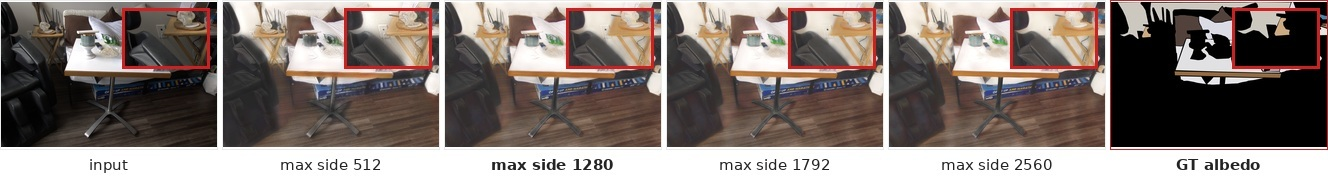
\includegraphics[width=\textwidth]{images/hires/maw_resolution.jpg}
  \caption[Inference-resolution comparison on MAW.]{%
    Effect of inference resolution on a MAW scene using the full-CARI model.
    The input photograph is shown on the left and the measured albedo on the
    right; the middle columns show predictions at different maximum side lengths.
    Each panel repeats the same black-sofa-armrest crop in the upper right with a red
    border to make blur differences easier to compare.
    Fine structure improves substantially from 512 to 1280 pixels, then largely
    plateaus. We therefore use the common 1280-pixel inference cap for every
    locally run MAW method; the official scorer subsequently reduces predictions
    to $320\times240$ before measuring the metrics.
  }
  \label{fig:maw_resolution}
\end{figure}

\paragraph{Benchmarks at a glance}
\figref{fig:datasets} previews the four evaluation benchmarks and the kind of
ground truth each provides, which determines the metric it supports
(\secref{sec:benchmarks}).
\figref{fig:comp_grid} shows the qualitative comparison format used throughout
this chapter: for a single in-the-wild image, the input and each method's
predicted albedo side by side.

\begin{figure}[t!]
  \centering
  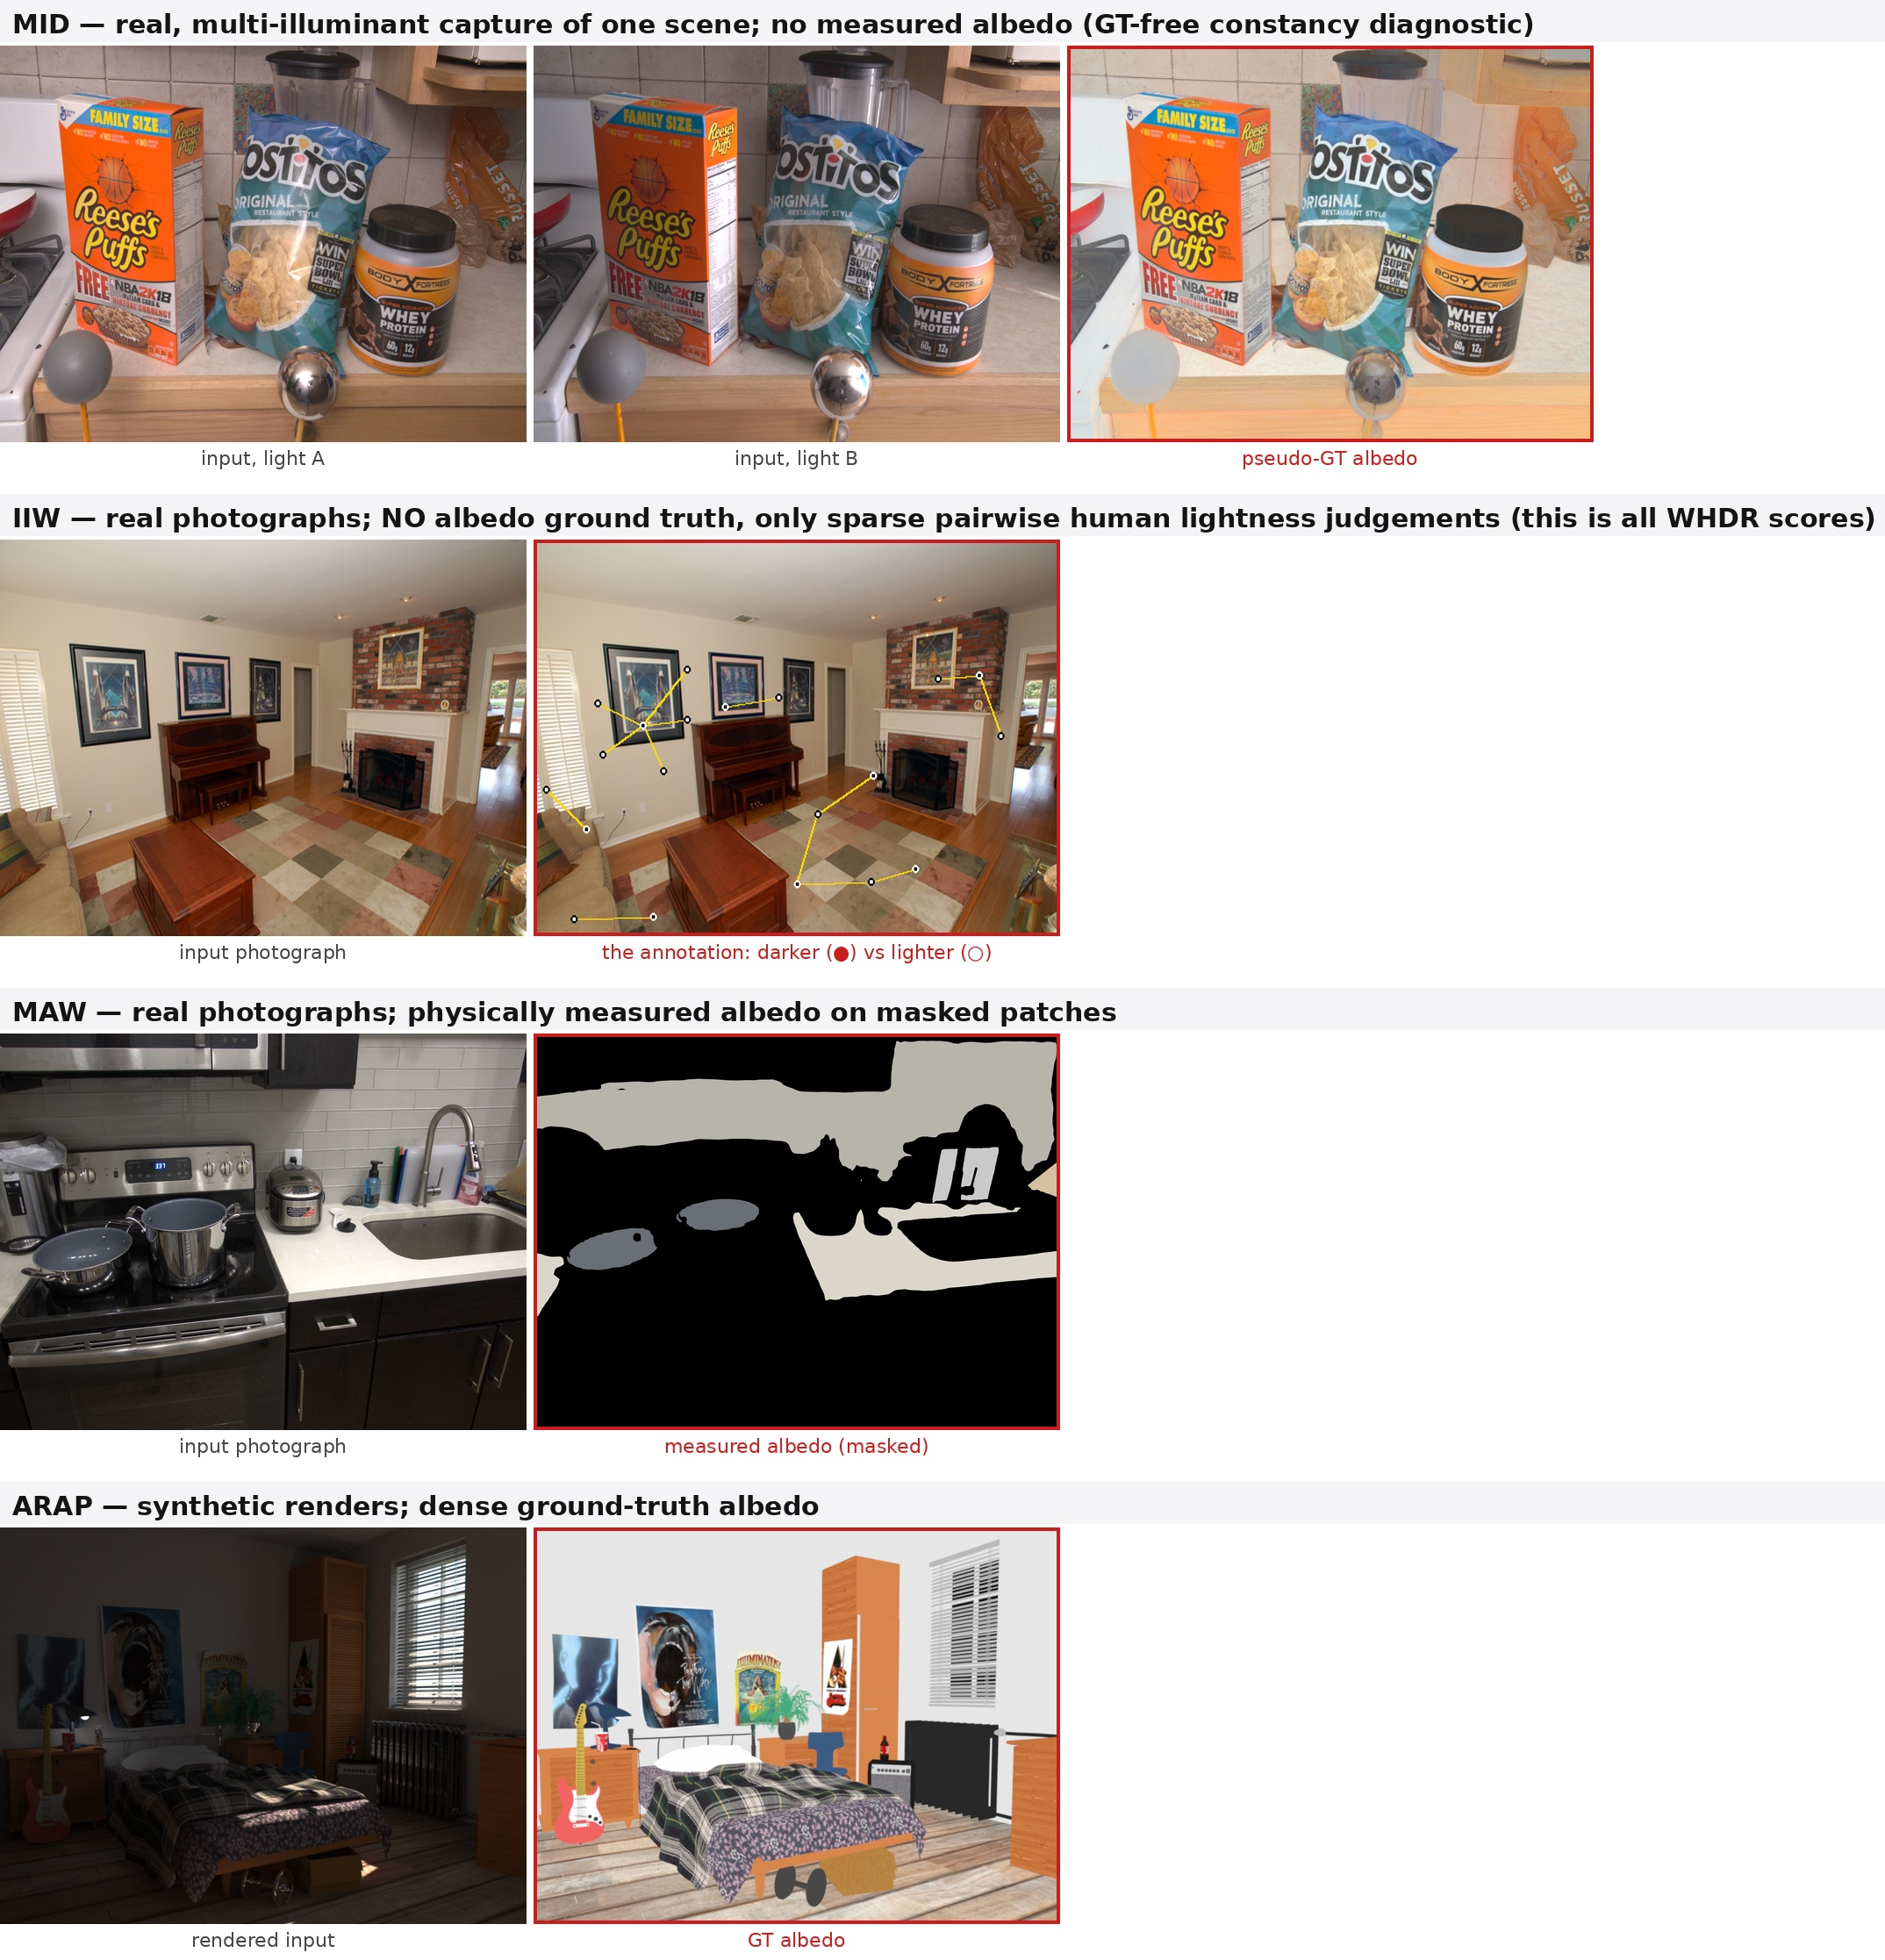
\includegraphics[width=0.92\textwidth]{images/datasets/datasets.jpg}
  \caption[The four evaluation benchmarks and their supervision.]{%
    The four evaluation benchmarks and the ground truth each provides, in the order the
    chapter presents them.
    \textbf{MID}: real multi-illuminant captures of one scene, with no measured albedo;
    which is why it supports a ground-truth-free constancy diagnostic and nothing stronger.
    \textbf{IIW}: real photographs with \emph{no} albedo ground truth at all. The second
    panel overlays the annotation that does exist: sparse pairwise human lightness
    judgements, each a pair of points one of which was called darker ($\bullet$) than the
    other ($\circ$). These sparse ordinal comparisons define what WHDR scores;
    they are informative about relative lightness but not RGB colour.
    \textbf{MAW}: real photographs with physically measured albedo on masked patches.
    \textbf{ARAP}: synthetic renders with dense ground-truth albedo.
  }
  \label{fig:datasets}
\end{figure}

\begin{figure}[t!]
  \centering
  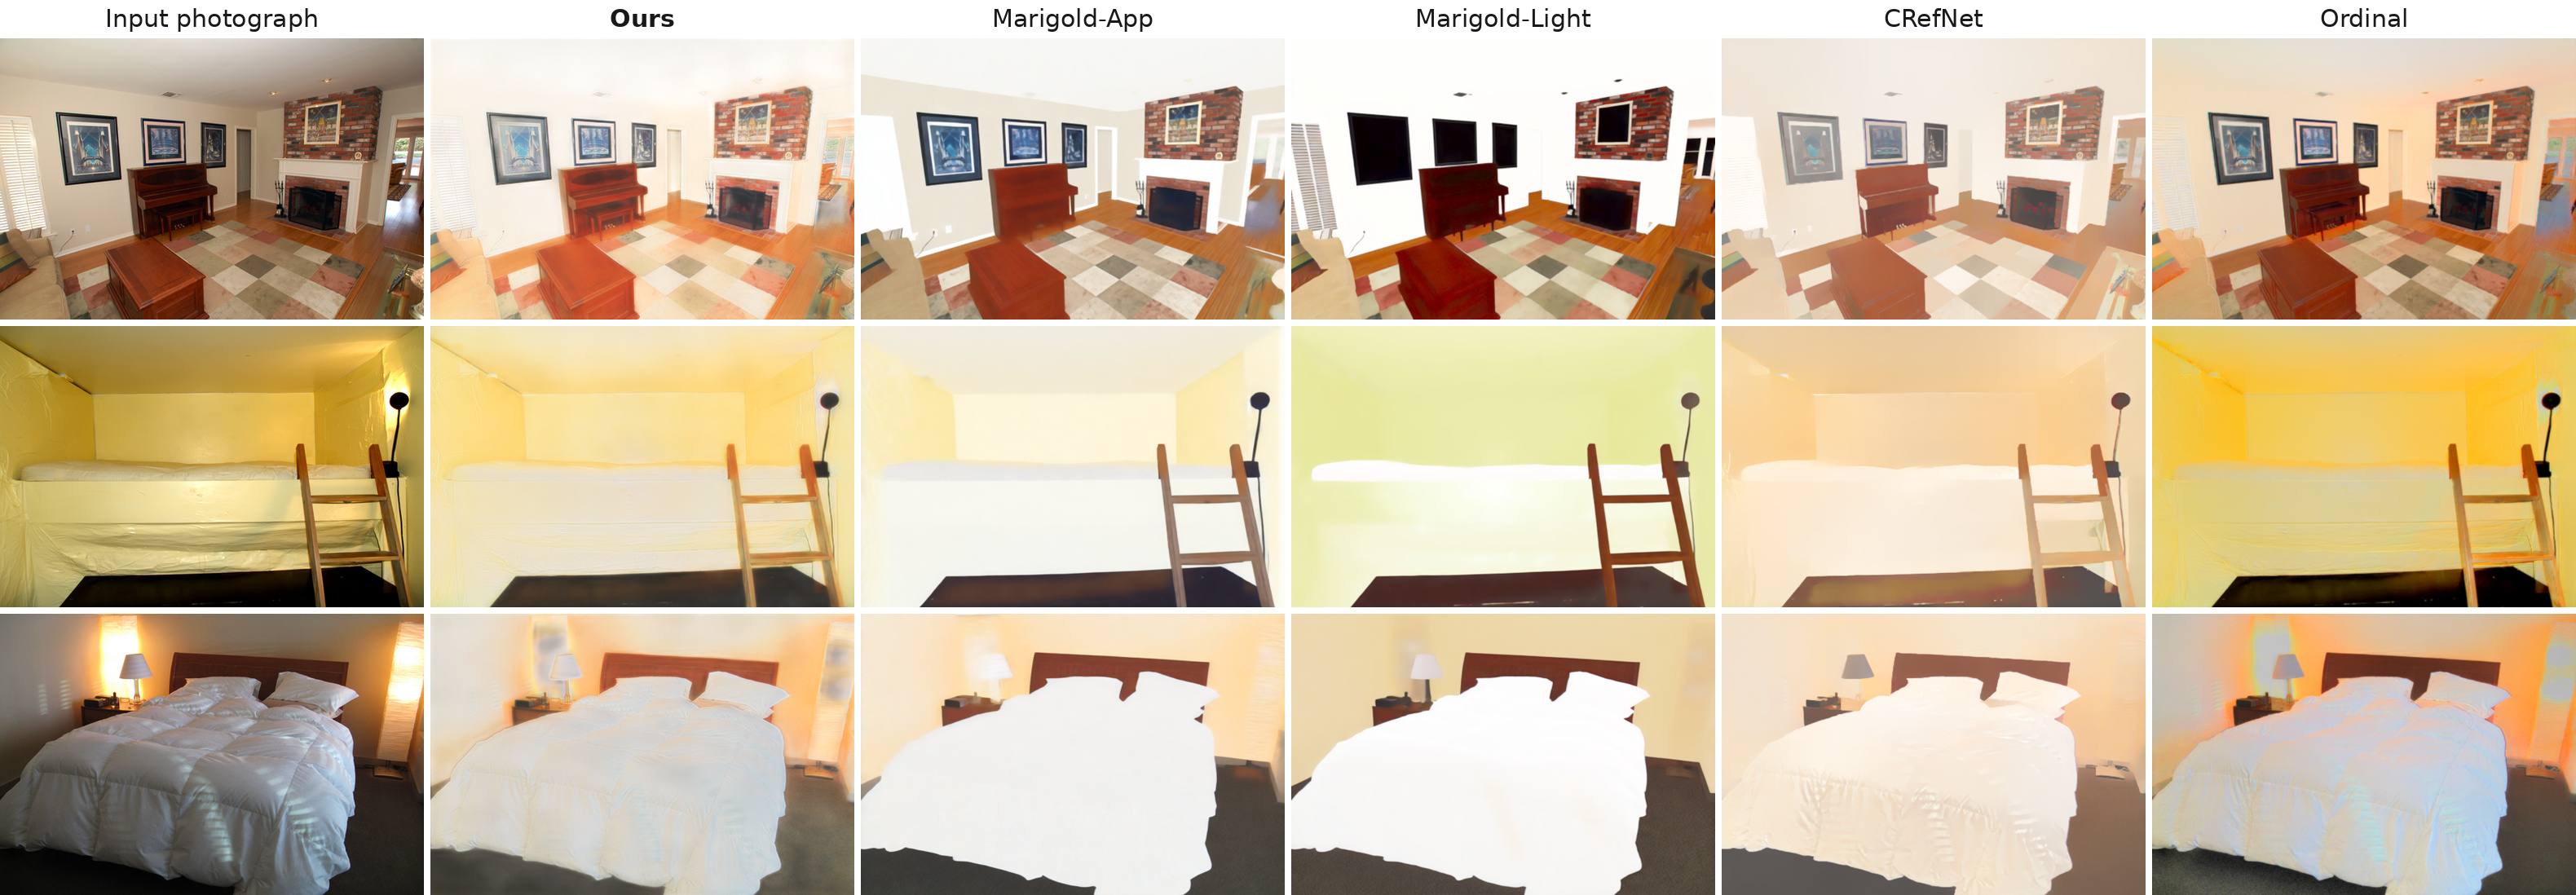
\includegraphics[width=\textwidth]{images/hires/comp_grid.jpg}
  \caption[Qualitative IIW albedo comparison across methods.]{%
    Qualitative albedo comparison on in-the-wild photographs (IIW), all methods run under
    the identical evaluation protocol. Each panel is scale-normalised by its own
    99th percentile, because albedo is defined only up to a global scale and each method
    fixes that scale differently; beyond this, no colour correction is applied.
    The comparison is deliberately shown, but it cannot be adjudicated: IIW supplies no
    albedo ground truth (\figref{fig:datasets}), so an albedo that looks ``cleaner'' cannot
    be distinguished by eye from one that has simply had its colour removed. The diffusion
    baselines whiten these interiors considerably more aggressively than we do, and on this
    evidence alone one might read that as a better decomposition. The MID pseudo-GT
    calibration in \tabref{tab:mid} shows the ambiguity: Marigold-App and CRefNet retain
    $72.8\%$ and $48.4\%$ of the reference chroma spread, against our $94.1\%$.
    This figure shows method behaviour; it cannot establish correctness on IIW.
  }
  \label{fig:comp_grid}
\end{figure}


\section{MID: Multi-Illuminant Constancy}
\label{sec:mid_results}

MIDIntrinsics \mycite{midintrinsics} photographs the same real room 25 times, moving
only the light, so it isolates the exact variable this thesis is about.
Because it ships no independently measured dense albedo, it cannot tell us whether a
prediction is \emph{correct}; it can only tell us whether a prediction is
\emph{stable}. That makes it a constancy diagnostic rather than an accuracy
benchmark, and we report it as such.
We use the held-out 30-scene test split. The two scores follow the
reflectance-consistency setting of \mycite{kinoshita21consistency} but are computed
directly on MID's illuminant groups.

Both scores rest on the same fact: within one scene, the material at a given pixel is
the same in every one of the 25 frames, so any variation in the predicted albedo
across frames is error by definition. Let $k = 1, \dots, N$ index the illuminant
conditions of a scene and let $m$ index the material regions given by the scene's
segmentation.

The first score asks whether the material's \emph{lightness} holds still.
Writing $\mu_{m,k}$ for the mean luminance of the predicted albedo over material $m$
in frame $k$, we take the coefficient of variation across frames and average it over
materials,
\begin{equation}
  C_{\text{mat}} \;=\;
  \frac{1}{|M|} \sum_{m \in M}
  \frac{\operatorname{std}_k\bigl(\mu_{m,k}\bigr)}
       {\operatorname{mean}_k\bigl(\mu_{m,k}\bigr)} .
  \label{eq:cmat}
\end{equation}
Dividing by the mean makes the score scale-free, which matters because albedo is only
defined up to a global scale.

The second score asks whether the material's \emph{colour} holds still, which is the
axis a coloured lamp actually attacks. We reduce each material in each frame to its
two chromaticity ratios $r_{m,k} = \bar{A}^{R}_{m,k} / \bar{A}^{G}_{m,k}$ and
$b_{m,k} = \bar{A}^{B}_{m,k} / \bar{A}^{G}_{m,k}$. Normalising by the green channel
removes brightness and leaves hue, so a model that lets a warm lamp tint its albedo
will show drift in $r_{m,k}$ and $b_{m,k}$ even if its lightness is stable.

\paragraph{Why the pooled chroma spread is not a constancy metric}
\label{par:castrms_correction}
The natural first move is to pool these ratios over every material and every frame and
report their combined spread,
\begin{equation}
  \text{Cast}_{\text{RMS}} \;=\;
  \sqrt{\operatorname{Var}\bigl(r_{m,k}\bigr) + \operatorname{Var}\bigl(b_{m,k}\bigr)} ,
  \label{eq:castrms}
\end{equation}
where the variance runs over all $(m,k)$ pairs jointly. This quantity is unsound as a
measure of illuminant invariance, and because it is easy to arrive at we set out
plainly why. By the law of total variance the pooled variance splits into
\begin{equation}
  \underbrace{\operatorname{Var}_{m,k}\bigl(r_{m,k}\bigr)}_{\text{pooled}}
  \;=\;
  \underbrace{\mathbb{E}_{m}\bigl[\operatorname{Var}_{k}(r_{m,k})\bigr]}_{\text{within: drift across illuminants}}
  \;+\;
  \underbrace{\operatorname{Var}_{m}\bigl(\mathbb{E}_{k}[r_{m,k}]\bigr)}_{\text{between: chroma spread across materials}} .
  \label{eq:castdecomp}
\end{equation}
Only the first term is the across-illuminant drift the metric is supposed to capture.
The second is the chromatic diversity of the \emph{scene}: a red sofa and a blue wall
genuinely differ in hue, and this diversity enters the pooled score even under perfect illuminant
invariance. It is tempting to dismiss it as a constant offset shared by every method
evaluated on a fixed scene set, but it is not model-independent: the between-material
term is computed from the \emph{predicted} albedo, so a model that pulls distinct
materials toward a common hue shrinks it, and thereby lowers
\eqnref{eq:castrms} without becoming any more illuminant-invariant.
\textbf{Pooling therefore rewards a model for destroying albedo colour.} This is not a
hypothetical defect: in \secref{sec:ablation} the configuration that scores best under
\eqnref{eq:castrms} is the one whose predicted albedo is visibly desaturated, and the
configuration that best preserves the MID pseudo-GT colour calibration is scored worst.

\paragraph{Reported chroma metrics}
We therefore report the two terms of \eqnref{eq:castdecomp} separately. Write the
per-material drift and the between-material chroma spread of a prediction $A$ as
\begin{equation}
  \delta_m \;=\; \sqrt{\operatorname{Var}_k(r_{m,k}) + \operatorname{Var}_k(b_{m,k})} ,
  \qquad
  S(A) \;=\; \sqrt{\operatorname{Var}_m\bigl(\bar{r}_m\bigr) + \operatorname{Var}_m\bigl(\bar{b}_m\bigr)} ,
  \label{eq:castterms}
\end{equation}
with $\bar{r}_m = \mathbb{E}_k[r_{m,k}]$ and $\bar{b}_m = \mathbb{E}_k[b_{m,k}]$. The
constancy score is the mean drift measured against the chroma scale the model actually
uses,
\begin{equation}
  \text{Cast}_{\text{rel}} \;=\;
  \frac{\tfrac{1}{|M|}\sum_{m \in M} \delta_m}{S(A)} ,
  \label{eq:castrel}
\end{equation}
a coefficient of variation in chroma. The normalisation is necessary because $\delta_m$
is an absolute quantity: a model that carries twice as much albedo chroma has twice as
much room to drift in absolute units, so comparing raw $\delta_m$ across models with
different colourfulness penalises the more colourful one for being colourful.
$\text{Cast}_{\text{rel}}$ instead asks the question that matters perceptually: whether
two materials remain distinguishable when the lighting changes.

Invariance alone, however, can never be reported on its own, because a constant
predictor attains it: a model that emits flat grey albedo is \emph{perfectly}
illuminant-invariant and scores zero on every drift measure. We therefore pair
\eqnref{eq:castrel} with a calibration guard measured against MID's dataset-derived
pseudo-ground-truth albedo. The
primary guard is the mean per-material chromaticity error,
\begin{equation}
  \text{Chroma}_{\text{err}} \;=\;
  \frac{1}{|M|}\sum_{m\in M}\bigl\lVert (\bar r_m,\bar b_m) - (\bar r^{*}_m,\bar b^{*}_m)\bigr\rVert,
  \label{eq:chromaerr}
\end{equation}
the distance between each predicted material's chromaticity and its pseudo-GT
chromaticity $(\bar r^{*}_m,\bar b^{*}_m)$; lower is better, and it is zero only when every
material matches that reference, not merely its amount of colour. Alongside it we
report a spread ratio,
\begin{equation}
  \text{Chroma}_{\text{fid}} \;=\; \frac{S(A)}{S(A^{*})} ,
  \label{eq:chromafid}
\end{equation}
where $A^{*}$ is the ground-truth albedo. This ratio is not a calibration score because a hue
permutation preserving the spread would score $1$. Instead, it is the specific detector of
\emph{collapse}: a model that greys its albedo drives $S(A)$, and hence
$\text{Chroma}_{\text{fid}}$, well below $1$, while an over-saturating model drives it above.
The two answer different questions and we report both: $\text{Chroma}_{\text{err}}$ asks
whether the colour is \emph{right}, $\text{Chroma}_{\text{fid}}$ whether it has been
\emph{destroyed}. A low $\text{Cast}_{\text{rel}}$ is a result only when it comes with a low
$\text{Chroma}_{\text{err}}$ and $\text{Chroma}_{\text{fid}} \approx 1$; achieved alongside
colour collapse it is the degenerate solution, not constancy. (We report
$\text{Chroma}_{\text{fid}}$ as the ratio of aggregate spreads rather than the mean of
per-scene ratios; the latter is inflated by a small number of low-chroma scenes and is not a
faithful summary.)

$C_{\text{mat}}$ and $\text{Cast}_{\text{rel}}$ are lower-is-better and both vanish for
a perfectly illuminant-invariant prediction. They are reported separately, rather than
combined, because they can move in opposite directions: $C_{\text{mat}}$ is a lightness
score and $\text{Cast}_{\text{rel}}$ a hue score, and a configuration may stabilise one
while disturbing the other.

This is deliberately an in-domain diagnostic: both our method and CD-IID train on the
disjoint MID training split \mycite{careaga24cdiid}. The table therefore compares
locally evaluated models under one pipeline and makes no zero-shot claim.

\begin{table}[t!]
  \caption[MID constancy and chroma calibration.]{%
    Multi-illuminant constancy on the held-out MIDIntrinsics test split
    \mycite{midintrinsics}, 30 scenes; brackets are $95\%$ percentile-bootstrap intervals
    over scenes. $C_{\text{mat}}$ (\eqnref{eq:cmat}) is lightness stability and
    $\text{Cast}_{\text{rel}}$ (\eqnref{eq:castrel}) is scale-normalised hue stability;
    lower is better for both. $\text{Chroma}_{\text{err}}$ (\eqnref{eq:chromaerr}, lower is
    better) is the primary colour-calibration guard (the distance of each predicted
    material's chromaticity from pseudo-GT), and $\text{Chroma}_{\text{fid}}$
    (\eqnref{eq:chromafid}, ratio of aggregate spreads, target $1$) is the collapse
    detector: below $1$ is greyed colour, above $1$ over-saturation. Gold, silver,
    and bronze mark first, second, and third numerical rank in each column;
    $\text{Chroma}_{\text{fid}}$ is ranked by absolute distance from its target of $1$,
    and displayed ties share a rank. The bootstrap intervals, rather than the colour fill,
    determine whether a difference is statistically supported. These are internal metrics, so no published method
    reports directly comparable values; the full CD-IID cascade is excluded because only its
    Ordinal Shading stage is integrated in our evaluation harness. $\dagger$ denotes the full
    model after IIW fine-tuning; this diagnostic row tests whether improving WHDR transfers to
    MID constancy and is not the selected model.
  }
  \label{tab:mid}
  \centering
  \small
  \resizebox{\textwidth}{!}{%
  \begin{tabular}{@{}lcccc@{}}
    \toprule
    Model & $C_{\text{mat}}$ $\downarrow$ & $\text{Chroma}_{\text{err}}$ $\downarrow$
          & $\text{Cast}_{\text{rel}}$ $\downarrow$ & $\text{Chroma}_{\text{fid}}$ ($\to 1$) \\
    \midrule
    Ours (full model)                          & \rankone{0.130\,{\scriptsize[.117,.144]}} & \rankone{0.121\,{\scriptsize[.102,.143]}} & 0.421\,{\scriptsize[.357,.485]} & \rankthree{0.941} \\
    Ours (IIW-fine-tuned)$^{\dagger}$          & 0.191\,{\scriptsize[.172,.211]} & \rankthree{0.134\,{\scriptsize[.115,.157]}} & 0.426\,{\scriptsize[.360,.493]} & \ranktwo{0.978} \\
    Ours (base CARI)                           & \rankthree{0.157\,{\scriptsize[.141,.174]}} & \ranktwo{0.129\,{\scriptsize[.109,.150]}} & 0.425\,{\scriptsize[.360,.491]} & \rankone{0.999} \\
    Marigold-App \mycite{marigoldiid24}        & 0.193\,{\scriptsize[.173,.214]} & 0.195\,{\scriptsize[.152,.245]} & \rankone{0.355\,{\scriptsize[.309,.406]}} & 0.728 \\
    Marigold-Light \mycite{marigoldiid24}      & 0.546\,{\scriptsize[.462,.645]} & 0.154\,{\scriptsize[.124,.187]} & \rankthree{0.392\,{\scriptsize[.333,.459]}} & 1.148 \\
    CRefNet \mycite{luo23crefnet}              & \ranktwo{0.151\,{\scriptsize[.138,.164]}} & 0.201\,{\scriptsize[.165,.241]} & \rankone{0.355\,{\scriptsize[.309,.406]}} & 0.484 \\
    Ordinal Shading \mycite{careaga23ordinal}  & 0.252\,{\scriptsize[.229,.279]} & 0.148\,{\scriptsize[.130,.166]} & 0.549\,{\scriptsize[.463,.637]} & 0.924 \\
    \bottomrule
  \end{tabular}}
\end{table}

\tabref{tab:mid} states the central result of this chapter, and it is a conjunction rather
than a victory on any single column. Two facts hold simultaneously, and the paired
bootstrap tells us which are real.

First, we do \emph{not} win illuminant invariance, and we say so first. Marigold-App and
CRefNet both attain $\text{Cast}_{\text{rel}} = 0.355$ against our $0.421$, and the paired
difference is significant in each case (\secref{sec:ablation} reports the intervals). On the
hue-stability axis in isolation, two external methods are genuinely more invariant than our
model.

Second, that ranking partly reflects what those methods discard. On the primary
calibration guard $\text{Chroma}_{\text{err}}$, which asks whether each material
matches MID's pseudo-GT hue rather than merely a stable one, our full model scores $0.121$ and
\emph{every} external method is significantly worse: CRefNet $0.201$, Marigold-App $0.195$,
Marigold-Light $0.154$, Ordinal $0.148$. The collapse detector explains the gap directly:
CRefNet retains under half the pseudo-GT between-material chroma spread
($\text{Chroma}_{\text{fid}} = 0.484$) and Marigold-App under three quarters ($0.728$),
whereas our model retains $94.1\%$ of it ($0.941$). A prediction cannot drift
in a dimension it has thrown away, so the two methods that lead $\text{Cast}_{\text{rel}}$
lead it partly by not carrying the colour that could vary.

The defensible claim is therefore narrow and, we think, stronger for it: our model is the
only one in the comparison that is best on lightness stability ($C_{\text{mat}}$,
significant over every other row), best on colour calibration ($\text{Chroma}_{\text{err}}$,
significant over every external method), and within a fifth of the most invariant method on
hue. Relative to Marigold this uses roughly $70\times$ fewer trainable parameters and about
one fifth of the inference time; relative to CRefNet it uses $3.6\times$ fewer trainable
parameters and is about $3\times$ faster (\tabref{tab:methods}). It is not the best
calibrated of our \emph{own} exploratory refinement rows
(two loss-refinement variants reach $\text{Chroma}_{\text{err}} = 0.115$); the refinement that buys
its lightness-stability and MAW advantages costs a little chroma calibration, and we report
that trade rather than hide it. The ablation of \secref{sec:ablation} demonstrates the
mechanism inside our own architecture: a configuration that collapses chroma to
$\text{Chroma}_{\text{fid}} = 0.55$ (almost exactly CRefNet's figure) is likewise
flattered by the superseded pooled score of \eqnref{eq:castrms}, and is visibly desaturated
to the eye.

\figref{fig:chroma_fidelity} makes that last point directly, because it is the one claim
in this chapter that can be checked without reference to any metric at all. Placed beside
the pseudo-GT albedo, the two predictions with the lowest pooled chroma cast, our own
colour-path-off configuration and CRefNet, are visibly drained of colour, while the
full model more closely follows the reference. The $\text{Chroma}_{\text{err}}$ and
aggregate spread ratio printed beneath each column quantify those properties.
A metric that ranks the first two of those images above the third is not measuring colour
constancy.

% Corrected MID trade-off scatter from rerun_mid_perscene.
% x = Cast_rel (lower is better); y = Chroma_err against MID pseudo-GT (lower is better).
\begin{figure}[t!]
  \centering
  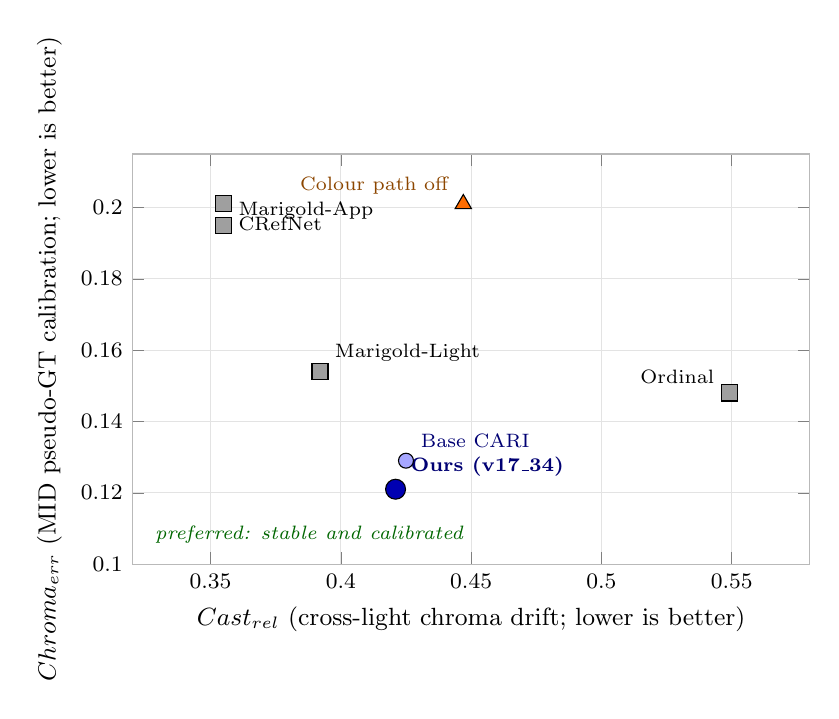
\begin{tikzpicture}
    \begin{axis}[
        width=0.84\textwidth, height=0.56\textwidth,
        xlabel={$\text{Cast}_{\text{rel}}$ (cross-light chroma drift; lower is better)},
        ylabel={$\text{Chroma}_{\text{err}}$ (MID pseudo-GT calibration; lower is better)},
        xlabel style={font=\small}, ylabel style={font=\small},
        tick label style={font=\footnotesize},
        xmin=0.32, xmax=0.58,
        ymin=0.10, ymax=0.215,
        grid=major,
        grid style={gray!22},
        axis line style={gray!55},
        clip=false,
      ]
      \node[anchor=south west, font=\scriptsize\itshape, text=green!40!black]
        at (axis cs:0.325,0.103) {preferred: stable and calibrated};

      \addplot[only marks, mark=*, mark size=3.6pt, draw=black, fill=blue!70!black]
        coordinates {(0.421,0.121)};
      \node[anchor=south west, font=\scriptsize\bfseries, blue!45!black]
        at (axis cs:0.423,0.122) {Ours (v17\_34)};

      \addplot[only marks, mark=*, mark size=2.7pt, draw=black, fill=blue!35]
        coordinates {(0.425,0.129)};
      \node[anchor=south west, font=\scriptsize, blue!45!black]
        at (axis cs:0.427,0.130) {Base CARI};

      \addplot[only marks, mark=triangle*, mark size=3.4pt, draw=black, fill=orange!85!red]
        coordinates {(0.447,0.201)};
      \node[anchor=south east, font=\scriptsize, orange!55!black]
        at (axis cs:0.445,0.201) {Colour path off};

      \addplot[only marks, mark=square*, mark size=2.9pt, draw=black, fill=gray!75]
        coordinates {(0.355,0.195) (0.392,0.154) (0.355,0.201) (0.549,0.148)};
      \node[anchor=south west, font=\scriptsize] at (axis cs:0.357,0.194) {Marigold-App};
      \node[anchor=south west, font=\scriptsize] at (axis cs:0.394,0.154) {Marigold-Light};
      \node[anchor=north west, font=\scriptsize] at (axis cs:0.357,0.200) {CRefNet};
      \node[anchor=south east, font=\scriptsize] at (axis cs:0.547,0.148) {Ordinal};
    \end{axis}
  \end{tikzpicture}
  \caption[MID constancy versus pseudo-GT chroma calibration.]{%
    Cross-light chroma stability against pseudo-GT chroma calibration on the
    30-scene MID test split. Lower is better on both axes. Marigold-App and
    CRefNet have lower drift but substantially higher calibration error; the
    selected model occupies a compromise region rather than winning either
    property universally. The companion spread diagnostic in
    \figref{fig:chroma_fidelity} shows whether low drift is accompanied by
    chroma collapse.
  }
  \label{fig:tradeoff}
\end{figure}


\figref{fig:tradeoff} plots stability against pseudo-GT calibration for the roster.
Lower is better on both axes. CRefNet and Marigold-App reduce drift more than our model,
but at substantially higher calibration error; the colour-path-off ablation occupies the
same high-error regime. The plot therefore exposes a trade-off rather than defining a
single winner.

\begin{figure}[t!]
  \centering
  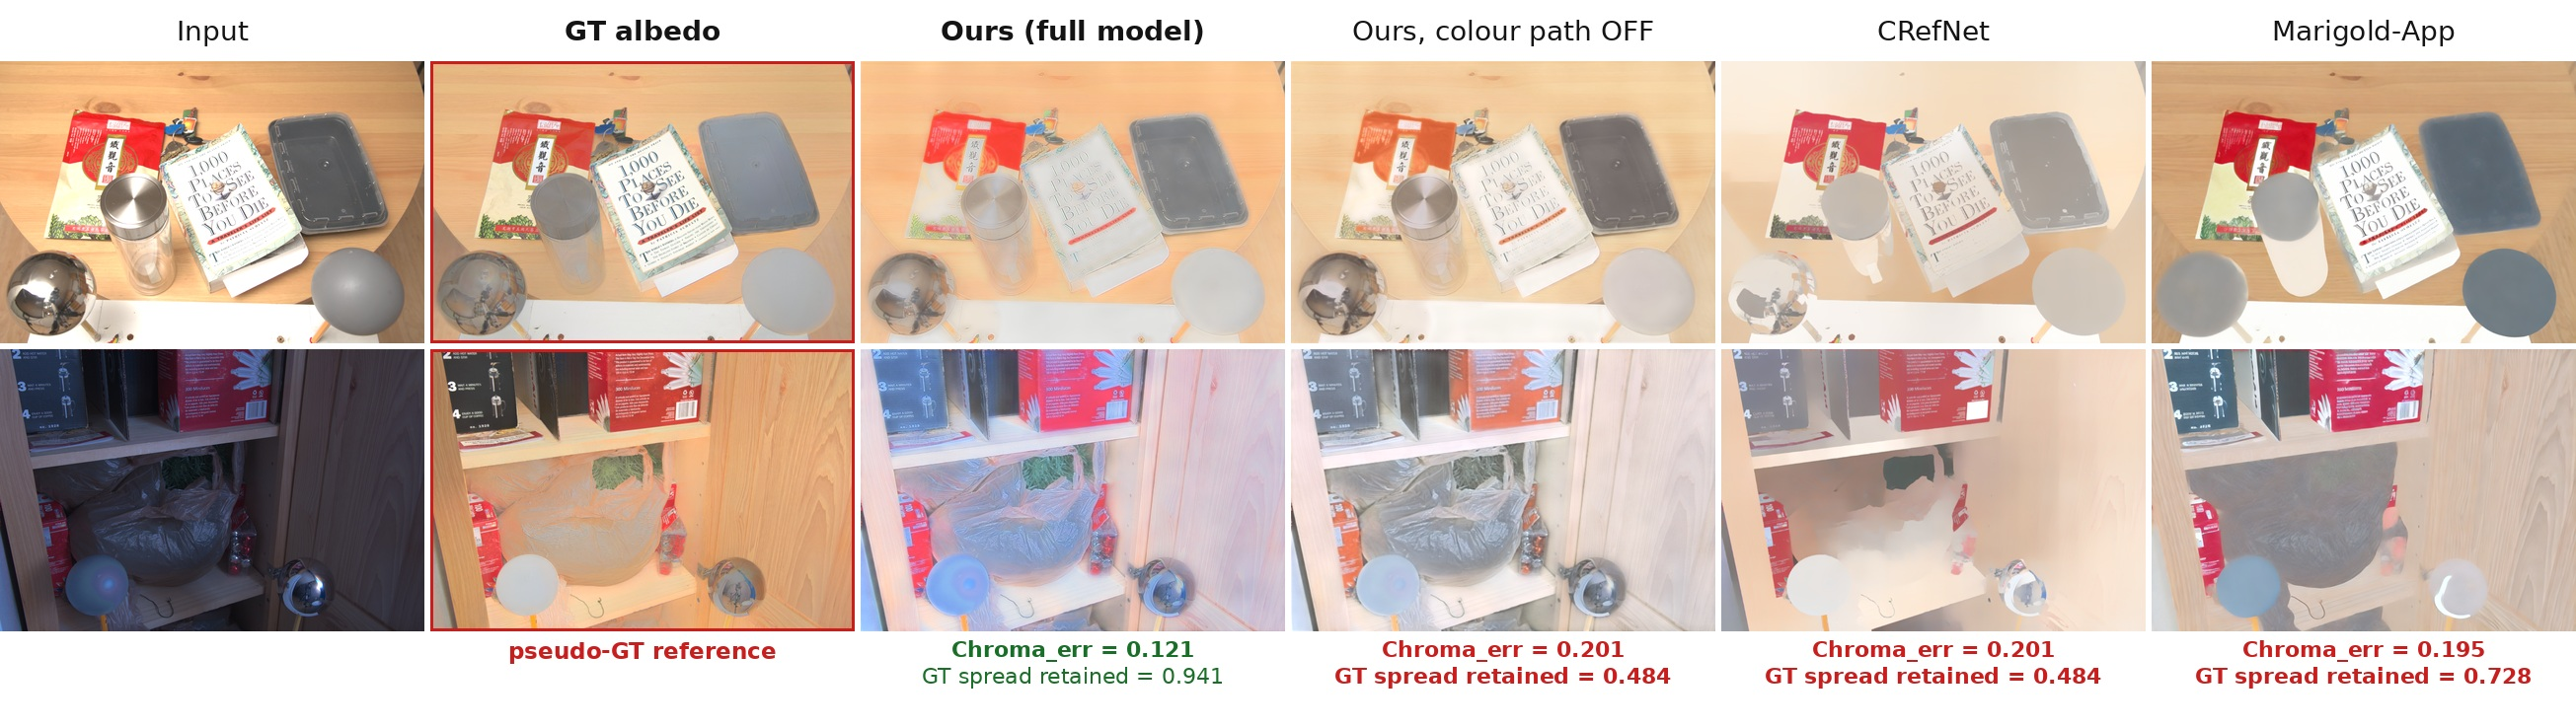
\includegraphics[width=\textwidth]{images/chroma_fidelity/chroma_fidelity.jpg}
  \caption[MID chroma calibration and spread-collapse diagnostic.]{%
    Chroma diagnostics on two distinct MIDIntrinsics test scenes and illuminant
    conditions (one row each). From left: the input, pseudo-GT albedo (red
    border), and four predictions. Albedo is defined only up to a global scale,
    so every panel is independently scale-normalised for display; no colour correction is applied,
    so the differences in saturation are differences in the predictions themselves.
    Values below each column are measured over the full 30-scene test split:
    $\text{Chroma}_{\text{err}}$ is the pseudo-GT calibration guard and the aggregate
    spread ratio diagnoses collapse. The colour-path-off row and CRefNet both retain
    $48.4\%$ of pseudo-GT chroma spread and have error 0.201, while the selected model
    retains $94.1\%$ with error 0.121.
  }
  \label{fig:chroma_fidelity}
\end{figure}

\figref{fig:mid_constancy} shows a qualitative comparison.
Each column is a different illuminant condition for the same scene.
Our model keeps the wall and floor colours consistent across columns;
Marigold-App shows a visible hue shift between the warm-light and cool-light
conditions.

\begin{figure}[t!]
  \centering
  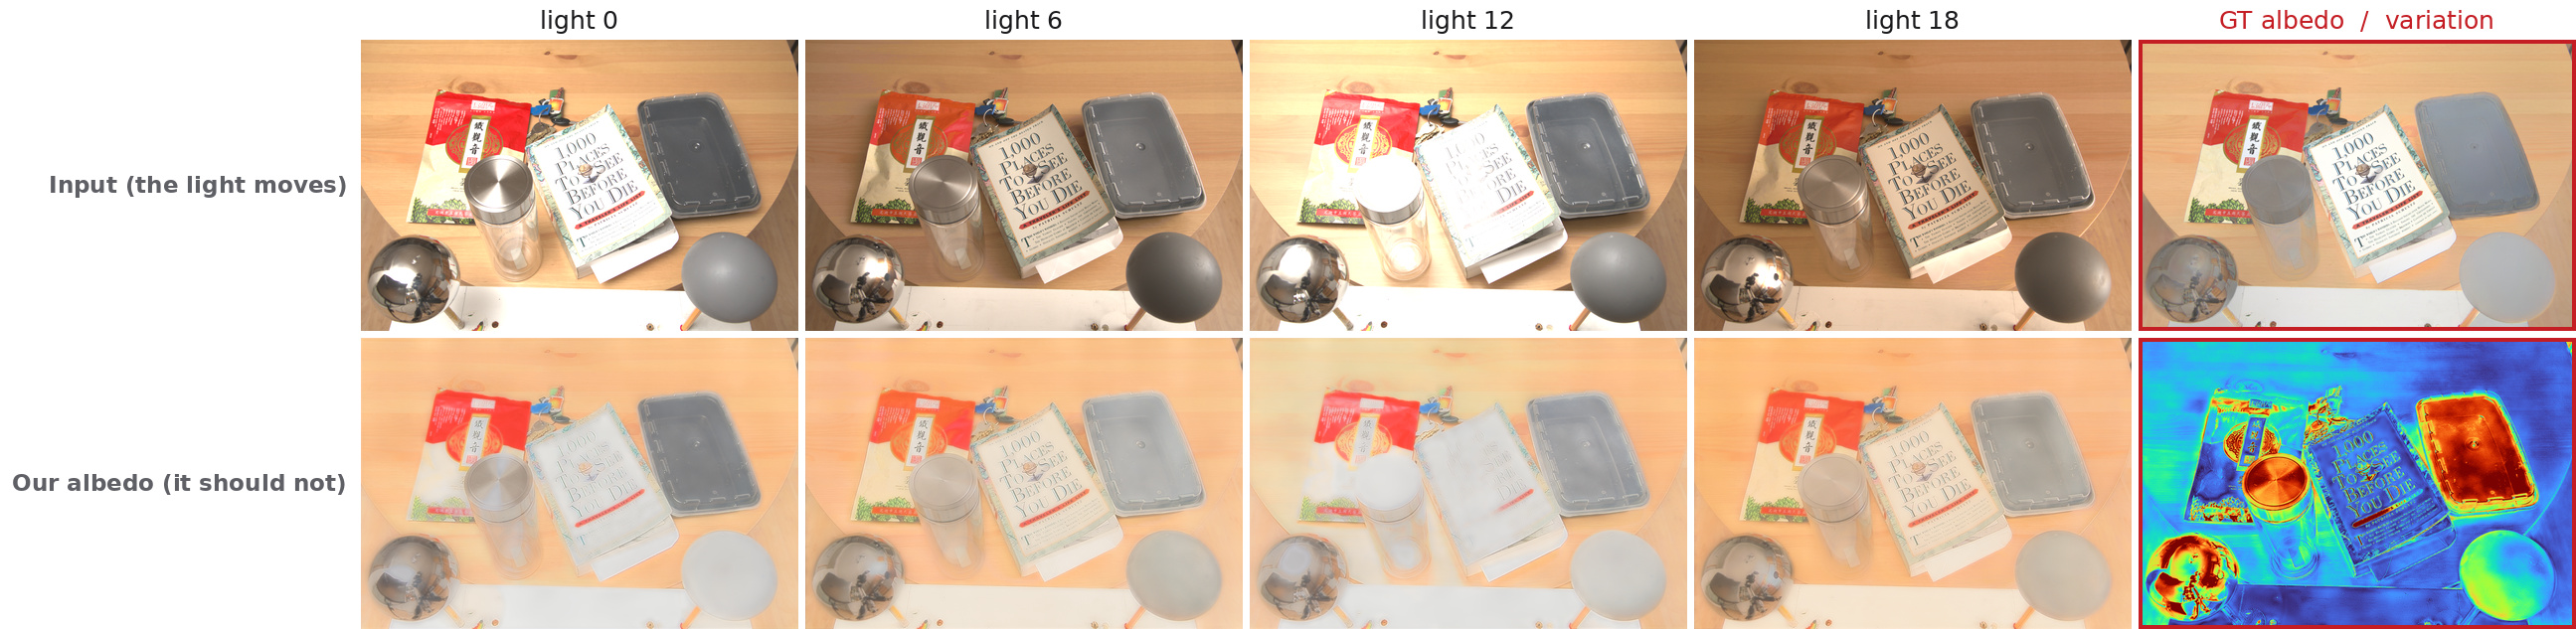
\includegraphics[width=\textwidth]{images/hires/mid_ours.jpg}
  \caption[MID albedo constancy under four illuminants.]{%
    Qualitative albedo constancy on one MID scene. The upper row shows four inputs
    and the pseudo-ground-truth albedo; the lower row shows the corresponding
    predictions and a per-pixel variation heatmap (red = the prediction changes
    with the light).
    The predicted material colours stay stable across illuminants, yielding cool
    (blue) CoV maps on the flat surfaces where the light changes most.
  }
  \label{fig:mid_constancy}
\end{figure}


\section{IIW: Perceptual Reflectance Ordering}
\label{sec:iiw_results}

IIW \mycite{bell14iiw} has been the default benchmark of the field for a decade,
so a decomposition method is expected to report it, and we do.
It scores a prediction with the Weighted Human Disagreement Rate (WHDR): human
annotators are shown two points in a photograph and asked which surface is
lighter, and WHDR is the confidence-weighted fraction of those comparisons that
the predicted albedo orders the wrong way,
\begin{equation}
  \text{WHDR} \;=\;
  \frac{\sum_{i} w_i \cdot \mathbb{1}\bigl[\hat{r}_i \neq r_i\bigr]}{\sum_{i} w_i},
  \label{eq:whdr}
\end{equation}
where $r_i$ is the human verdict on the $i$-th pair (lighter, darker, or equal),
$\hat{r}_i$ is the verdict implied by the predicted albedo under a threshold on the
ratio of the two points' intensities, and $w_i$ is the annotator confidence.
Lower is better.

\eqnref{eq:whdr} is worth writing out because its limitations are visible in it.
The comparison $\hat{r}_i$ depends only on the \emph{ratio} of two predicted
intensities, so WHDR is invariant to any global rescaling of the albedo and, more
importantly, it never looks at colour at all: the albedo is reduced to a lightness
ordering before it is scored.
A model can therefore tint every surface in the image with the colour of the lamp
and lose nothing on this metric, as long as the relative lightness of surface pairs
survives.
Its labels are sparse and perceptual, resting on human judgements rather than a
physical albedo measurement. Subjectivity is not inherently a weakness: when
the intended property is perceived relative reflectance, people are the
appropriate observers. The limitation is one of \emph{scope}. A sparse ordinal
lightness label cannot determine absolute intensity, chromaticity, or texture,
so complementary metrics are needed for those properties
\mycite{maw,sato25metrics}.

This matters directly for the claim of this thesis. Coloured illuminant leakage is
a \emph{hue} error, and \eqnref{eq:whdr} is hue-blind by construction, so WHDR
cannot confirm or refute the property we are trying to improve. We therefore report
it as complementary evidence: it tests whether enforcing colour constancy damages
the relative reflectance ordering that viewers care about, but it cannot validate
the coloured-illumination claim by itself.
The benchmark that does address material colour directly is MAW, which
\secref{sec:maw_results} turns to next and which was created for exactly this gap
\mycite{maw}.

\tabref{tab:iiw} separates locally evaluated rows from cited full-split context.
Supervision status is stated explicitly because the local block contains both zero-shot
models and models trained on IIW. The cited numbers are not used as a head-to-head
comparison with our local rows: each source has its own inference implementation and
training protocol.

\begin{table}[t!]
  \caption[IIW WHDR results.]{%
    Results on IIW \mycite{bell14iiw}. WHDR is lower-is-better. The upper block
    is evaluated locally; rows using IIW supervision are identified explicitly. The first cited block is selected
    no-IIW-supervision rows from Ordinal Shading \mycite{careaga23ordinal},
    Table~2. The second is the full-IIW roster reproduced by Wang et al.
    \mycite{yuan25texture}, Table~I, an arXiv preprint that evaluates all
    5,230 IIW images with per-method recommended settings. Repeated methods are
    intentional: they expose source- and protocol-dependent reported values,
    not a unified rerun. Both cited blocks are context rather than a head-to-head
    comparison with our local split. $\dagger$ denotes IIW fine-tuning: the
    \emph{Ours (IIW-fine-tuned)} row is our full model fine-tuned on the IIW training split (the
    complement of this test split, so no leakage), and its WHDR is therefore not zero-shot.
    Its number is \emph{italicised, not bolded}, because it is bought at a cost the WHDR
    column cannot see: fine-tuning for WHDR degrades MID lightness constancy
    ($C_{\text{mat}}$) by $47\%$ (\tabref{tab:mid} baseline $0.130\!\to\!0.191$), which is
    precisely the antagonism \secref{sec:mid_results} predicts and the reason we do not adopt
    it as the headline model.
  }
  \label{tab:iiw}
  \centering
  \small
  \begin{tabular}{@{}lc@{}}
    \toprule
    Model & WHDR $\downarrow$ \\
    \midrule
    Ours (full model) & 0.264 \\
    Ours (base CARI) & 0.286 \\
    Ours (IIW-fine-tuned)$^{\dagger}$ & \textit{0.220} \\
    Marigold-App \mycite{marigoldiid24} & 0.193 \\
    Marigold-Light \mycite{marigoldiid24} & 0.215 \\
    CRefNet (local; IIW-supervised) \mycite{luo23crefnet} & \textbf{0.168} \\
    Ordinal (local) \mycite{careaga23ordinal} & 0.257 \\
    \midrule
    \multicolumn{2}{@{}l}{\itshape\small Cited from Ordinal Shading, Table~2 (no IIW supervision):}\\
    Bell et al. \mycite{bell14iiw} & 0.206 \\
    CGIntrinsics \mycite{li18cgintrinsics} & 0.178 \\
    NIID-Net \mycite{luo20niid} & 0.166 \\
    PIE-Net \mycite{das22pienet} & 0.213 \\
    Ordinal Shading \mycite{careaga23ordinal} & 0.249 \\
    \midrule
    \multicolumn{2}{@{}l}{\itshape\small Full IIW test split, Wang et al., Table~I:}\\
    Bell et al. \mycite{bell14iiw} & 0.206 \\
    CGIntrinsics \mycite{li18cgintrinsics} & 0.154 \\
    NIID-Net \mycite{luo20niid} & 0.166 \\
    CRefNet \mycite{luo23crefnet} & 0.145 \\
    Texture-aware IID \mycite{yuan25texture} & 0.136 \\
    \midrule
    \multicolumn{2}{@{}l}{\itshape\small Original CRefNet result (different protocol):}\\
    CRefNet$^\dagger$ \mycite{luo23crefnet} & 0.108 \\
    \bottomrule
  \end{tabular}
\end{table}

The \emph{Ours (IIW-fine-tuned)} row makes the mismatch concrete rather than rhetorical. Fine-tuning
our full model on the IIW training split with the ordinal-hinge loss does what it is asked
to do: WHDR falls from $0.264$ to $0.220$. The accuracy and lightness-constancy guards
regress in exchange, all past the pre-specified $10\%$ no-regression threshold. The damage is
heaviest on \emph{lightness}: MID $C_{\text{mat}}$ rises from $0.130$ to $0.191$ ($+47\%$)
and MAW intensity error from $0.624$ to $1.057$ ($+69\%$). This is the expected signature because
WHDR is an ordinal \emph{lightness} score and optimising it reshapes lightness stability
first. But it is not confined there: MAW $\Delta E$, measured against \emph{physically
measured} albedo, worsens from $3.981$ to $5.163$ ($+30\%$), so colour accuracy degrades too,
even though the in-domain MID hue-drift and chroma-collapse guards remain comparatively stable
($\text{Chroma}_{\text{err}}$ $0.121\!\to\!0.134$, $\text{Chroma}_{\text{fid}}$
$0.941\!\to\!0.978$, and $\text{Cast}_{\text{rel}}$ $0.421\!\to\!0.426$), which reminds us
that the external measured reference is the stricter test.
The shape of the trade differs from the chroma collapse by which the feed-forward baselines
reach low chroma cast (\secref{sec:mid_results}). There the casualty is hue; here it is chiefly
lightness. The lesson is nevertheless identical: improving one scalar benchmark can hide
failures that only complementary guards expose. We report the fine-tuned row for completeness and as this
demonstration, not as the selected model: the WHDR gain is real, but it does not serve our
stated objective because it is bought at the expense of the constancy the thesis aims to
protect.

\figref{fig:iiw} shows qualitative results on the IIW test set, and illustrates the
mismatch between what the metric rewards and what this thesis is optimising.

\begin{figure}[t!]
  \centering
  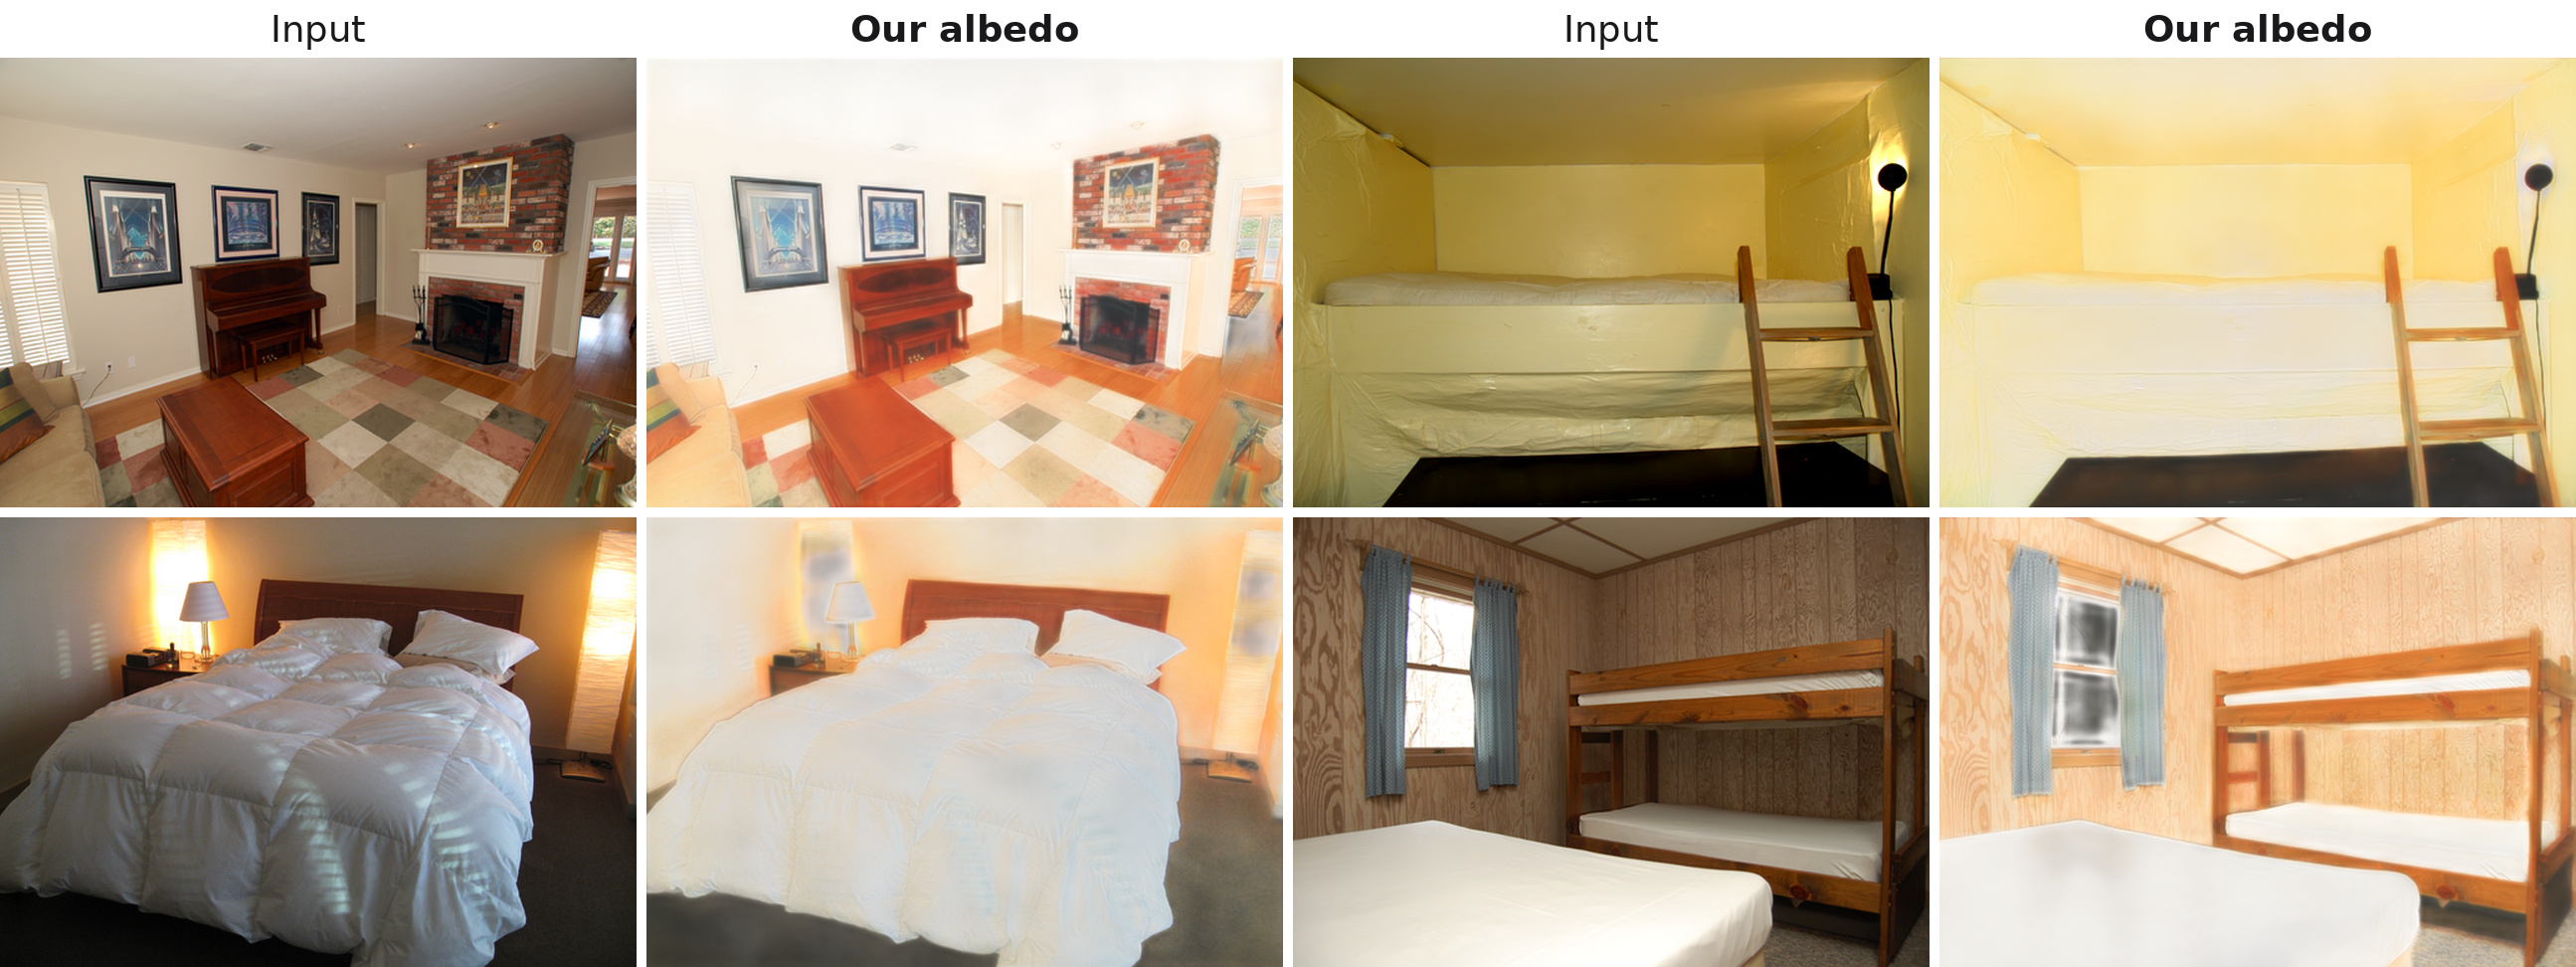
\includegraphics[width=0.85\textwidth]{images/hires/iiw_ours.jpg}
  \caption[IIW qualitative predictions and failure cases.]{%
    Qualitative albedo predictions from our model on IIW test images.
    Each row shows an input image (left) and its predicted albedo (right).
    The predictions preserve broad material regions but show the two competing
    errors that an ordinal score can expose only at annotated point pairs:
    legitimate material boundaries may be over-smoothed, while illumination
    structure remains on the ceiling and around the windows. This figure is an
    honest failure case rather than evidence of colour accuracy, because IIW
    provides no measured RGB albedo.
  }
  \label{fig:iiw}
\end{figure}


\section{MAW: Measured Real-World Albedo}
\label{sec:maw_results}

MAW \mycite{maw} was built to close the gap that \secref{sec:iiw_results} just
described.
Instead of asking people which of two patches looks lighter, its authors recover a
physical albedo value for real surfaces.
They photograph a surface twice, once with a grey card of known reflectance resting
on it and once without.
Both the surface and the card receive the same illumination, so the shading term is
shared and cancels in the ratio of the two measurements, which leaves the surface's
albedo in absolute terms.
The ground truth is therefore a measured quantity rather than a perceptual vote,
which makes MAW the benchmark best able to answer the question this thesis poses:
when a real room is lit by a coloured light, does the predicted material colour match
the material's real colour?

Because that ground truth is measured rather than derived from the prediction, MAW scores
colour \emph{correctness} against an external reference, not merely stability across
conditions. Both metrics remove the global-scale ambiguity: $\Delta E$ is computed on
chromaticity, while the intensity error is explicitly scale-invariant. MAW therefore measures the right \emph{chromaticity} and
the right \emph{relative} brightness, not an absolute radiometric value.
It is thus complementary to MID rather than a substitute for it: a model can be
perfectly stable across illuminants (a low $C_{\text{mat}}$) and still be
consistently wrong about what colour the wall is, and MAW is what catches that.

The public scorer first resizes the prediction and region mask to $320\!\times\!240$
and extracts a robust median RGB vector $\hat{\mathbf a}_m$ for each measured material
region $m$; $\mathbf a_m^\star$ is the corresponding measured reference and $w_m$ is
the region area. Let $\ell(\mathbf x)=\tfrac{1}{3}\sum_c x_c$ denote the scorer's
RGB channel mean. The colour score removes intensity independently for each material,
$\beta_m=\ell(\mathbf a_m^\star)/\ell(\hat{\mathbf a}_m)$, and reports the area-weighted
CIEDE2000 colour difference,
\begin{equation}
  \Delta E_{00} =
  \frac{\sum_m w_m\,
  \Delta E_{00}\!\left(\mathrm{Lab}(\beta_m\hat{\mathbf a}_m),
  \mathrm{Lab}(\mathbf a_m^\star)\right)}{\sum_m w_m}.
  \label{eq:deltae}
\end{equation}
This per-material scale alignment makes the score primarily a chromaticity test rather
than a test of recovered intensity. It is therefore the primary external score for a
coloured-illuminant leak.

The second score tests relative material brightness. Writing
$\hat l_m=\ell(\hat{\mathbf a}_m)$ and $l_m^\star=\ell(\mathbf a_m^\star)$, the scorer fits
one area-weighted global scale
\begin{equation}
  \alpha^\star =
  \frac{\sum_m w_m\hat l_m l_m^\star}
       {\sum_m w_m\hat l_m^2},
  \qquad
  \text{SI-MSE} =
  \frac{\sum_m w_m(\alpha^\star\hat l_m-l_m^\star)^2}{\sum_m w_m}.
  \label{eq:simse}
\end{equation}
Because the scale is fitted away, this score is insensitive to a uniformly too-dark
or too-bright prediction and instead penalises the wrong \emph{relative} lightness of
different materials. It does not directly measure spatial blur, although smoothing can
change the robust region medians on which it is computed.

We run every local method with the common 1280-pixel long-side inference cap specified
in \secref{sec:exp_setup}; the public scorer then performs its fixed $320\!\times\!240$
evaluation and scale handling, matching the MAW protocol used by CD-IID
\mycite{careaga24cdiid}.

\tabref{tab:maw} reports $\Delta E$, the CIELAB colour difference between the
prediction and measured albedo, and intensity SI-MSE$\times100$, which removes
the global-scale ambiguity before assessing brightness. Lower is better for
both. The cited block is retained only for methods reported under the same MAW
protocol, with CD-IID Table~1 as the primary external reference.

\begin{table}[t!]
  \caption[MAW albedo accuracy results.]{%
    Results on MAW \mycite{maw}, evaluated with the benchmark scorer.
    $\Delta E$ measures CIELAB colour difference and intensity
    SI-MSE$\times100$ measures scale-invariant brightness error; lower is
    better for both. The upper block is evaluated locally. The complete lower
    block is transcribed from CD-IID \mycite{careaga24cdiid}, Table~1. $\dagger$ marks the
    diagnostic full model after IIW fine-tuning; it is included to expose cross-benchmark
    damage and is not the selected model.
    $^{*}$ denotes the grayscale-shading assumption, for which predicted
    chromaticity is inherited from the input image. Gold, silver, and bronze
    cells mark first, second, and third place over the common protocol.
  }
  \label{tab:maw}
  \centering
  \small
  \begin{tabular}{@{}lcc@{}}
    \toprule
    Model & $\Delta E$ $\downarrow$ & Int. SI-MSE$\times$100 $\downarrow$ \\
    \midrule
    Ours (full model)                          & 3.981 & 0.624 \\
    Ours (IIW-fine-tuned)$^{\dagger}$          & 5.163 & 1.057 \\
    Ours (base CARI)                           & 4.155 & \rankthree{0.504} \\
    Ours (colour path only; Table-A Row~3)     & 4.115 & \rankone{0.395} \\
    Marigold-App \mycite{marigoldiid24}        & \ranktwo{3.775} & 0.653 \\
    Marigold-Light \mycite{marigoldiid24}      & 4.214 & \ranktwo{0.493} \\
    CRefNet \mycite{luo23crefnet}              & \rankthree{3.970} & 0.942 \\
    Ordinal (local) \mycite{careaga23ordinal}  & 6.884 & 0.657 \\
    \midrule
    \multicolumn{3}{@{}l}{\itshape\small Cited from CD-IID, Table~1:}\\
    Bell et al. \mycite{bell14iiw}             & 6.61 & 3.11 \\
    CGIntrinsics \mycite{li18cgintrinsics}     & 5.15 & 2.71 \\
    Li \& Snavely (2018a)$^{*}$ \mycite{li18bigtime} & 6.56 & 1.72 \\
    NIID-Net \mycite{luo20niid}                & 4.73 & 1.24 \\
    IRISformer \mycite{zhu22irisformer}        & 4.94 & 1.44 \\
    Kocsis et al. \mycite{kocsis24iid}         & 5.35 & 1.13 \\
    IntrinsicAnything \mycite{chen24intrinsicanything} & 4.12 & 0.98 \\
    Ordinal Shading$^{*}$ \mycite{careaga23ordinal} & 6.56 & 0.57 \\
    CD-IID \mycite{careaga24cdiid}             & \rankone{3.37} & 0.54 \\
    \bottomrule
  \end{tabular}
\end{table}

The IIW-fine-tuned diagnostic confirms the trade-off with an independent measured reference.
Its $17\%$ WHDR improvement is accompanied by a $30\%$ increase in MAW $\Delta E$ and a
$69\%$ increase in intensity error. The effect is therefore not confined to MID's
dataset-derived pseudo-ground truth: direct optimisation of the sparse ordinal objective also
damages colour and relative intensity against physically measured albedo.

\figref{fig:maw} shows a representative MAW scene.
The ground-truth panel is masked to the surface regions whose albedo was
physically measured by the dataset authors; only those regions enter the
score.

\begin{figure}[t!]
  \centering
  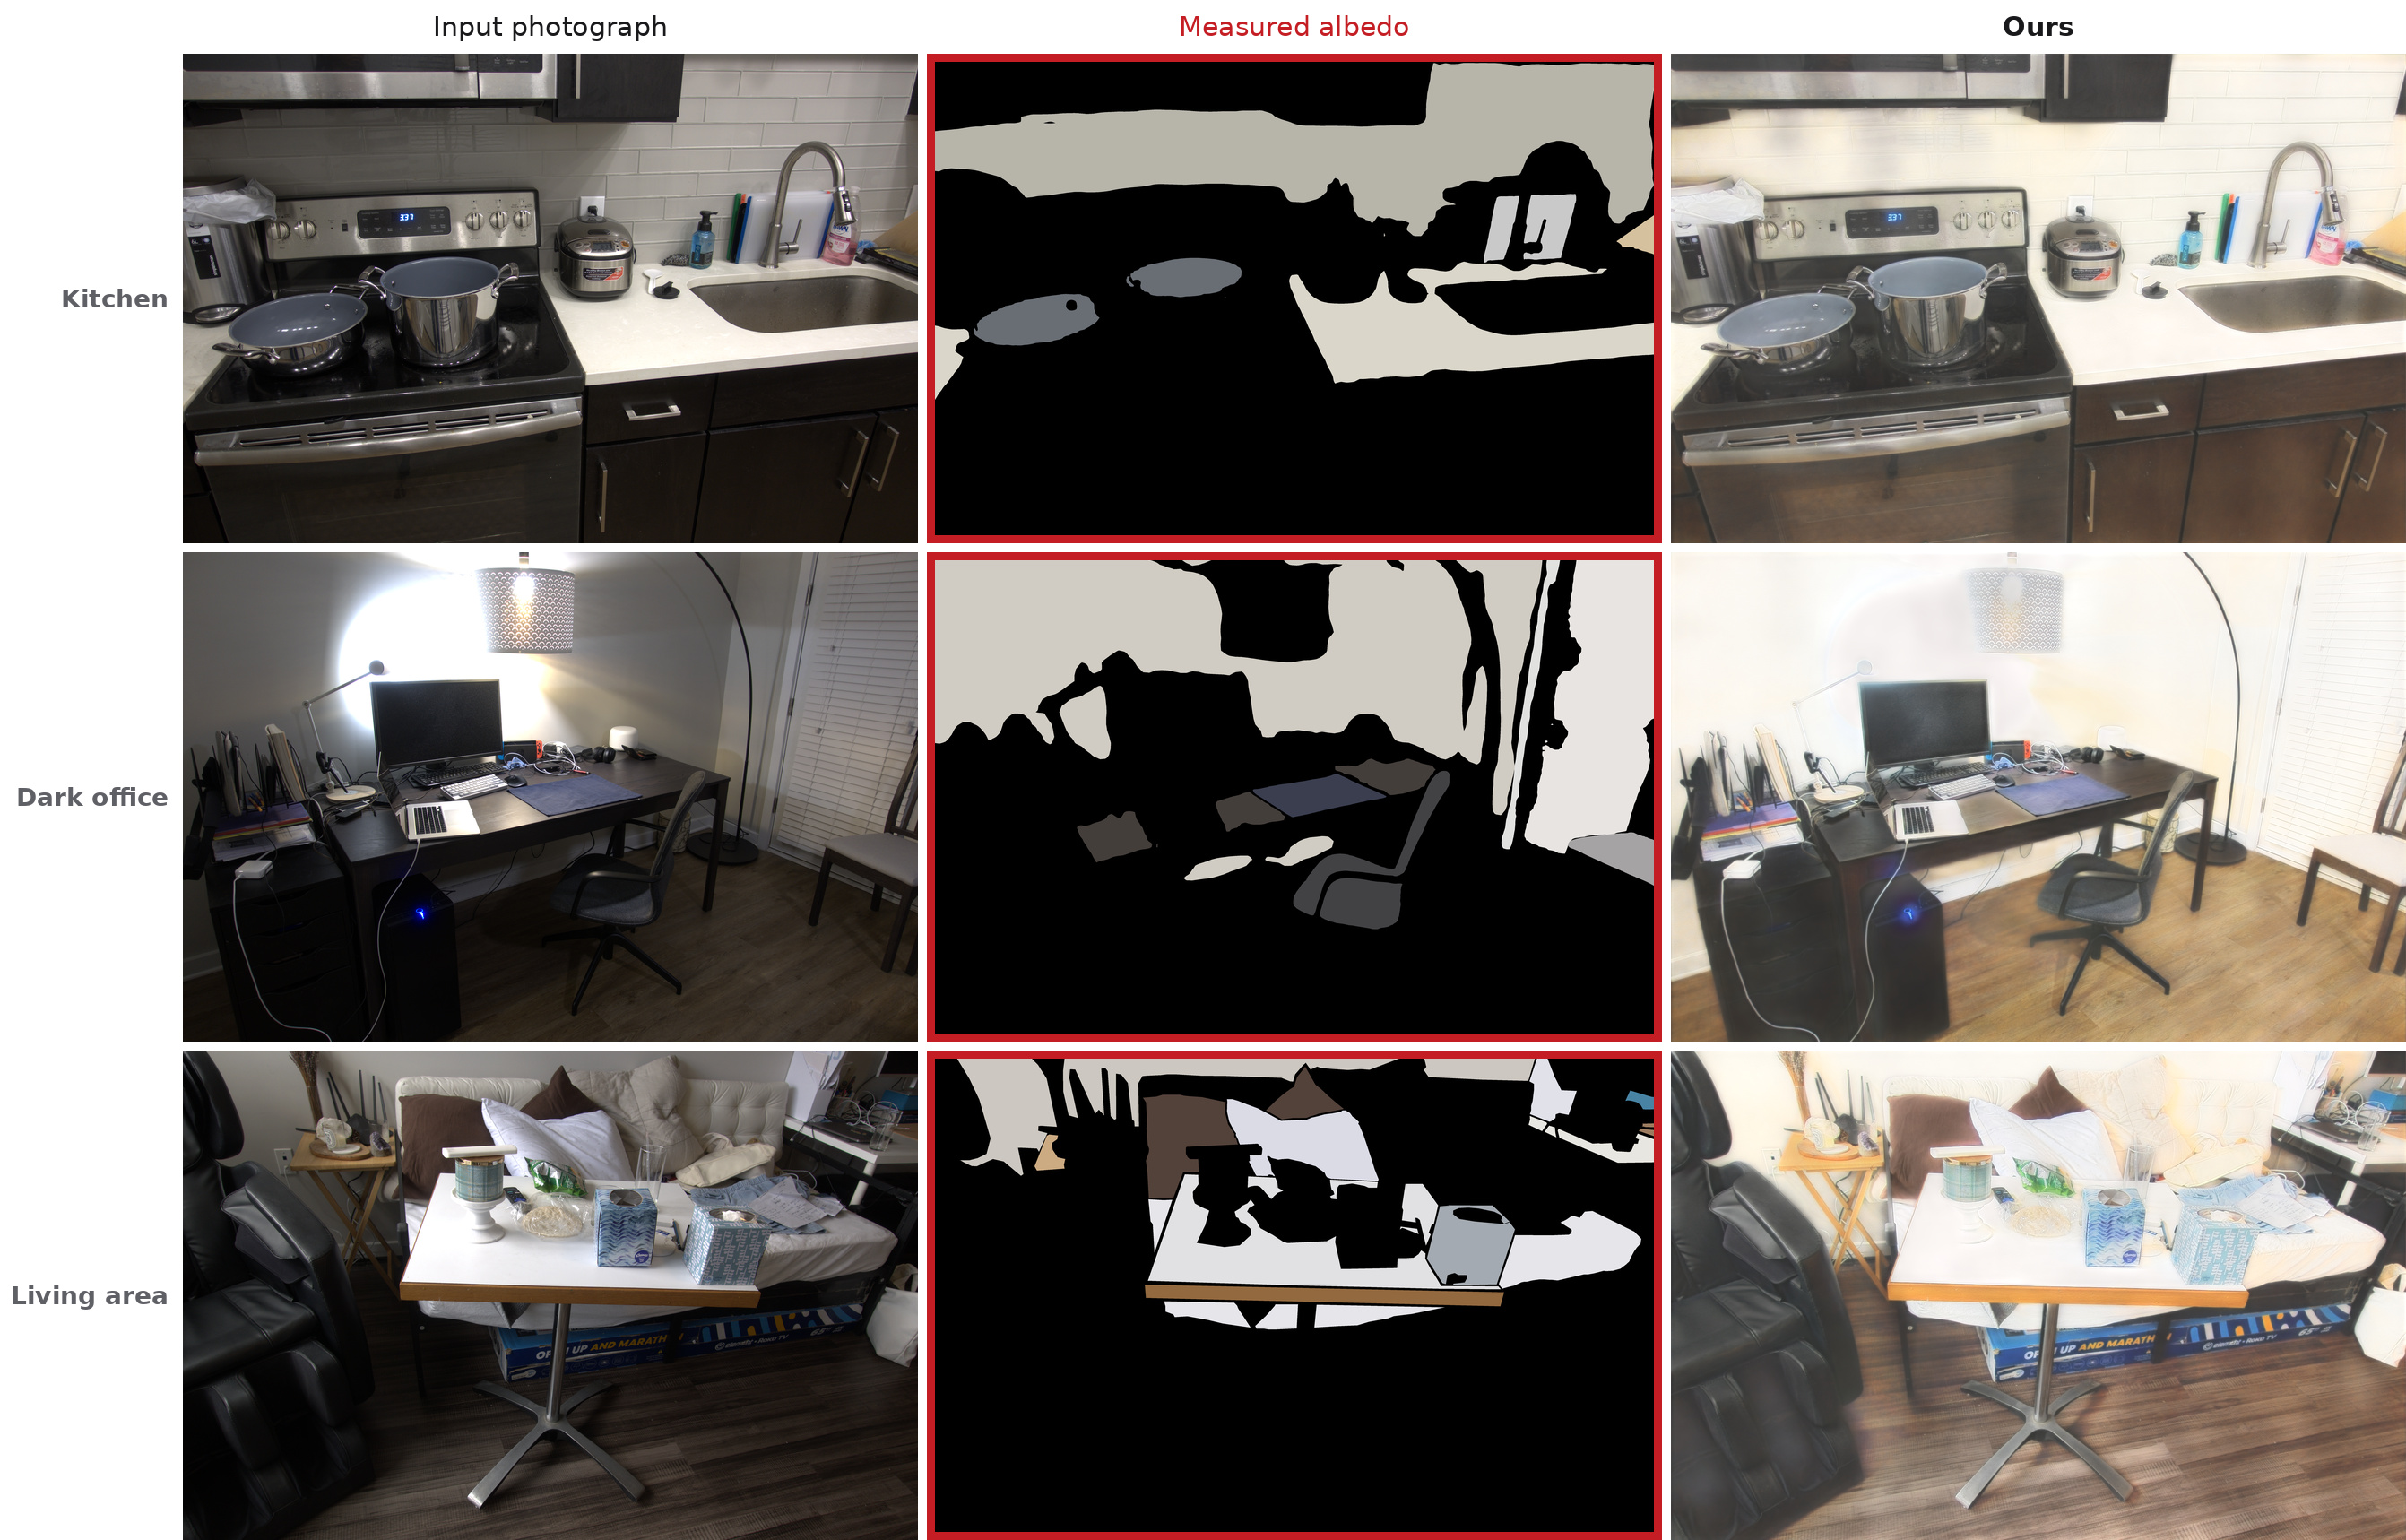
\includegraphics[width=\textwidth]{images/hires/maw_ours.jpg}
  \caption[Qualitative MAW albedo comparison.]{%
    Qualitative comparison on three content-diverse MAW photographs (one per
    row): a kitchen, a dark office, and a living area. Left to right: input
    photograph, measured albedo (red border and masked to reliable regions),
    and the prediction from Ours. All three middle panels show the corresponding
    physically measured MAW albedo mask.
  }
  \label{fig:maw}
\end{figure}


\section{ARAP: Constancy and Albedo Accuracy}
\label{sec:arap_results}

ARAP \mycite{arap} is synthetic, and we report it last for that reason: a rendered
scene is an easier target than a photograph, so a good ARAP number cannot by itself
support a claim about real rooms.
What ARAP uniquely offers is that it is the only benchmark here with dense
ground-truth albedo \emph{and} several renderings of the same scene under different
lights. MID has the repeated illuminants but no true albedo; MAW has the true albedo
but only one illuminant per surface. ARAP has both, so it is the one place where
constancy and accuracy can be measured on the very same pixels, and where a claim
that improving one damages the other can actually be tested.

It answers two distinct questions, which must not be merged.
First, does a prediction stay stable when the original coloured illumination changes?
This is tested on the raw renderings with our self-consistency measures
(\tabref{tab:arap_constancy}).
Second, how accurate is the recovered albedo when the input is neutrally lit?
This is tested on white-balanced input against dense ground-truth albedo
(\tabref{tab:arap_accuracy}).

We white-balance correctly, which is worth stating because an earlier version of our
evaluator did not. A single global exposure rescale (multiplying all three channels by
one scalar) leaves the chromaticity of the illuminant untouched and is therefore
\emph{not} white balance; measured on a coloured-lit ARAP scene it leaves the implied
illuminant as far from neutral after the operation as before. We instead reconstruct an
achromatic-illuminant image from the ground-truth albedo: writing the implied shading as
$\mathbf{S}=\mathbf{I}/\mathbf{A}^{*}$, we recompose $\mathbf{I}_{\text{wb}} =
\mathbf{A}^{*}\cdot\mathrm{lum}(\mathbf{S})$, which drives the implied illuminant chromaticity
to exactly neutral. The accuracy table uses this reconstruction; the constancy table uses the
raw coloured renderings, since removing the illuminant would erase the very variable the
constancy measure exists to probe.

Two coverage points follow. The constancy table
(\tabref{tab:arap_constancy}) is restricted to the multi-illuminant groups whose illuminant
\emph{colour} actually changes between renderings ($16$ groups overall, $11$ indoor): cross-light
drift is undefined for a single-light scene, and groups that vary only intensity or direction
carry no colour cast for an invariant albedo to be tested against, so including them would pull
every model's score toward zero and mask the effect the thesis is about. The accuracy table
(\tabref{tab:arap_accuracy}) instead scores every image with usable dense albedo, namely 136 of
the 157 in the collection; the other 21 have near-black ground truth (fewer than 88 valid
pixels) and are dropped deterministically for every model alike. The accuracy
table combines our local white-balanced evaluation with published original-ARAP
results from Ordinal Shading \mycite{careaga23ordinal}, Table~1.

\begin{table}[t!]
  \caption[ARAP cross-illumination constancy.]{%
    ARAP raw-input constancy on the \emph{colour-varying} groups of the original ARAP
    collection \mycite{arap} --- the groups in which the illuminant \emph{colour} changes
    between renderings, which is the literal case this thesis is about ($16$ groups overall,
    $11$ indoor; the remaining multi-light groups vary only intensity/direction and are
    excluded, since they carry no colour for the albedo to be invariant to and would dilute
    the score toward zero). $C_{\text{arap}}$ measures cross-illumination albedo variation and
    $\text{Cast}_{\text{RMS}}$ residual chroma-cast variation; lower is better for every
    column. Gold, silver, and bronze mark first, second, and third numerical rank in each
    column; displayed ties share a rank. These are internal diagnostics, evaluated locally.
  }
  \label{tab:arap_constancy}
  \centering
  \resizebox{\textwidth}{!}{%
  \begin{tabular}{@{}lcccc@{}}
    \toprule
    & \multicolumn{2}{c}{All colour-varying ($n{=}16$)}
      & \multicolumn{2}{c}{Indoor colour-varying ($n{=}11$)} \\
    \cmidrule(lr){2-3}\cmidrule(l){4-5}
    Model & $C_{\text{arap}}$ $\downarrow$ & $\text{Cast}_{\text{RMS}}$ $\downarrow$
          & $C_{\text{arap}}$ $\downarrow$ & $\text{Cast}_{\text{RMS}}$ $\downarrow$ \\
    \midrule
    Ours (full model)                          & \rankthree{0.142} & \ranktwo{\textit{0.079}} & \rankone{0.096} & \ranktwo{\textit{0.077}} \\
    Ours (base CARI)                           & 0.154 & \rankthree{\textit{0.092}} & \rankthree{0.119} & \rankthree{\textit{0.094}} \\
    Marigold-App \mycite{marigoldiid24}        & \rankone{0.113} & \rankone{\textit{0.052}} & \ranktwo{0.113} & \rankone{\textit{0.038}} \\
    Marigold-Light \mycite{marigoldiid24}      & 0.340 & \textit{0.197} & 0.340 & \textit{0.256} \\
    CRefNet \mycite{luo23crefnet}              & \ranktwo{0.128} & \textit{0.122} & 0.129 & \textit{0.137} \\
    Ordinal Shading \mycite{careaga23ordinal}  & 0.175 & \textit{0.294} & 0.165 & \textit{0.355} \\
    \bottomrule
  \end{tabular}}\\[3pt]
  {\footnotesize $\text{Cast}_{\text{RMS}}$ is shown in \textit{italics}.
  Its rank colours indicate numerical order only, not a stand-alone quality claim.
  Unlike the MID pooled score it carries no between-material term. It is a chroma
  variance taken across the illuminants of a single scene, but it remains an
  \emph{absolute} variance, which a colourless albedo minimises just as effectively as an
  invariant one. It is reported for completeness and read against the chroma-fidelity
  figures of \tabref{tab:mid}: the methods that lead this column are the same ones that
  retain the least albedo chroma. $C_{\text{arap}}$ is also a pure constancy score and
  can be minimised by a constant prediction; it must be read beside the dense-GT accuracy
  guard in \tabref{tab:arap_accuracy}.}
\end{table}

\begin{table}[t!]
  \caption[ARAP dense-albedo accuracy.]{%
    ARAP albedo accuracy, \emph{within-study}, on the full Bonneel et al. collection
    \mycite{arap} (136 of 157 images have dense ground-truth albedo with enough valid
    pixels to score; the same 136 are used for every model). Input is white-balanced by
    reconstructing an achromatic-illuminant image from the ground-truth albedo
    (\secref{sec:arap_results}). LMSE and mean-normalised RMSE are lower-is-better, SSIM
    higher. The upper block is evaluated locally under one harness; the lower
    block is transcribed from Ordinal Shading \mycite{careaga23ordinal},
    Table~1. Gold, silver, and bronze mark first, second, and third place
    across all rows.
  }
  \label{tab:arap_accuracy}
  \centering
  \small
  \begin{tabular}{@{}lccc@{}}
    \toprule
    Model & LMSE $\downarrow$ & mn-RMSE $\downarrow$ & SSIM $\uparrow$ \\
    \midrule
    Ours (full model)                          & 0.0275 & \ranktwo{0.2150} & \ranktwo{0.8083} \\
    Ours (base CARI)                           & 0.0279 & \rankthree{0.2259} & \rankthree{0.8067} \\
    Marigold-App \mycite{marigoldiid24}        & 0.0266 & 0.2529 & 0.8016 \\
    Marigold-Light \mycite{marigoldiid24}      & 0.0706 & 0.6187 & \rankone{0.8204} \\
    CRefNet \mycite{luo23crefnet}              & 0.0223 & 0.2916 & 0.8051 \\
    \midrule
    \multicolumn{4}{@{}l}{\itshape\small Published original-ARAP protocol (Ordinal Shading, Table~1):}\\
    Chromaticity \mycite{arap}                 & 0.024 & 0.296 & 0.692 \\
    NIID-Net \mycite{luo20niid}                & \rankthree{0.022} & \rankone{0.206} & 0.781 \\
    Li \& Snavely \mycite{li18bigtime}         & \rankone{0.018} & 0.227 & 0.749 \\
    Bell et al.\ \mycite{bell14iiw}            & 0.028 & 0.317 & 0.718 \\
    PIE-Net \mycite{das22pienet}               & 0.026 & 0.273 & \rankthree{0.754} \\
    Ordinal Shading \mycite{careaga23ordinal}  & \ranktwo{0.021} & 0.252 & 0.761 \\
    \bottomrule
  \end{tabular}
\end{table}

\figref{fig:arap_models} provides the model-by-illuminant comparison that the
aggregate tables cannot show spatially. \figref{fig:arap_constancy} then samples
three distinct ARAP interiors to reduce dependence on that single scene.

\begin{figure}[p!]
  \centering
  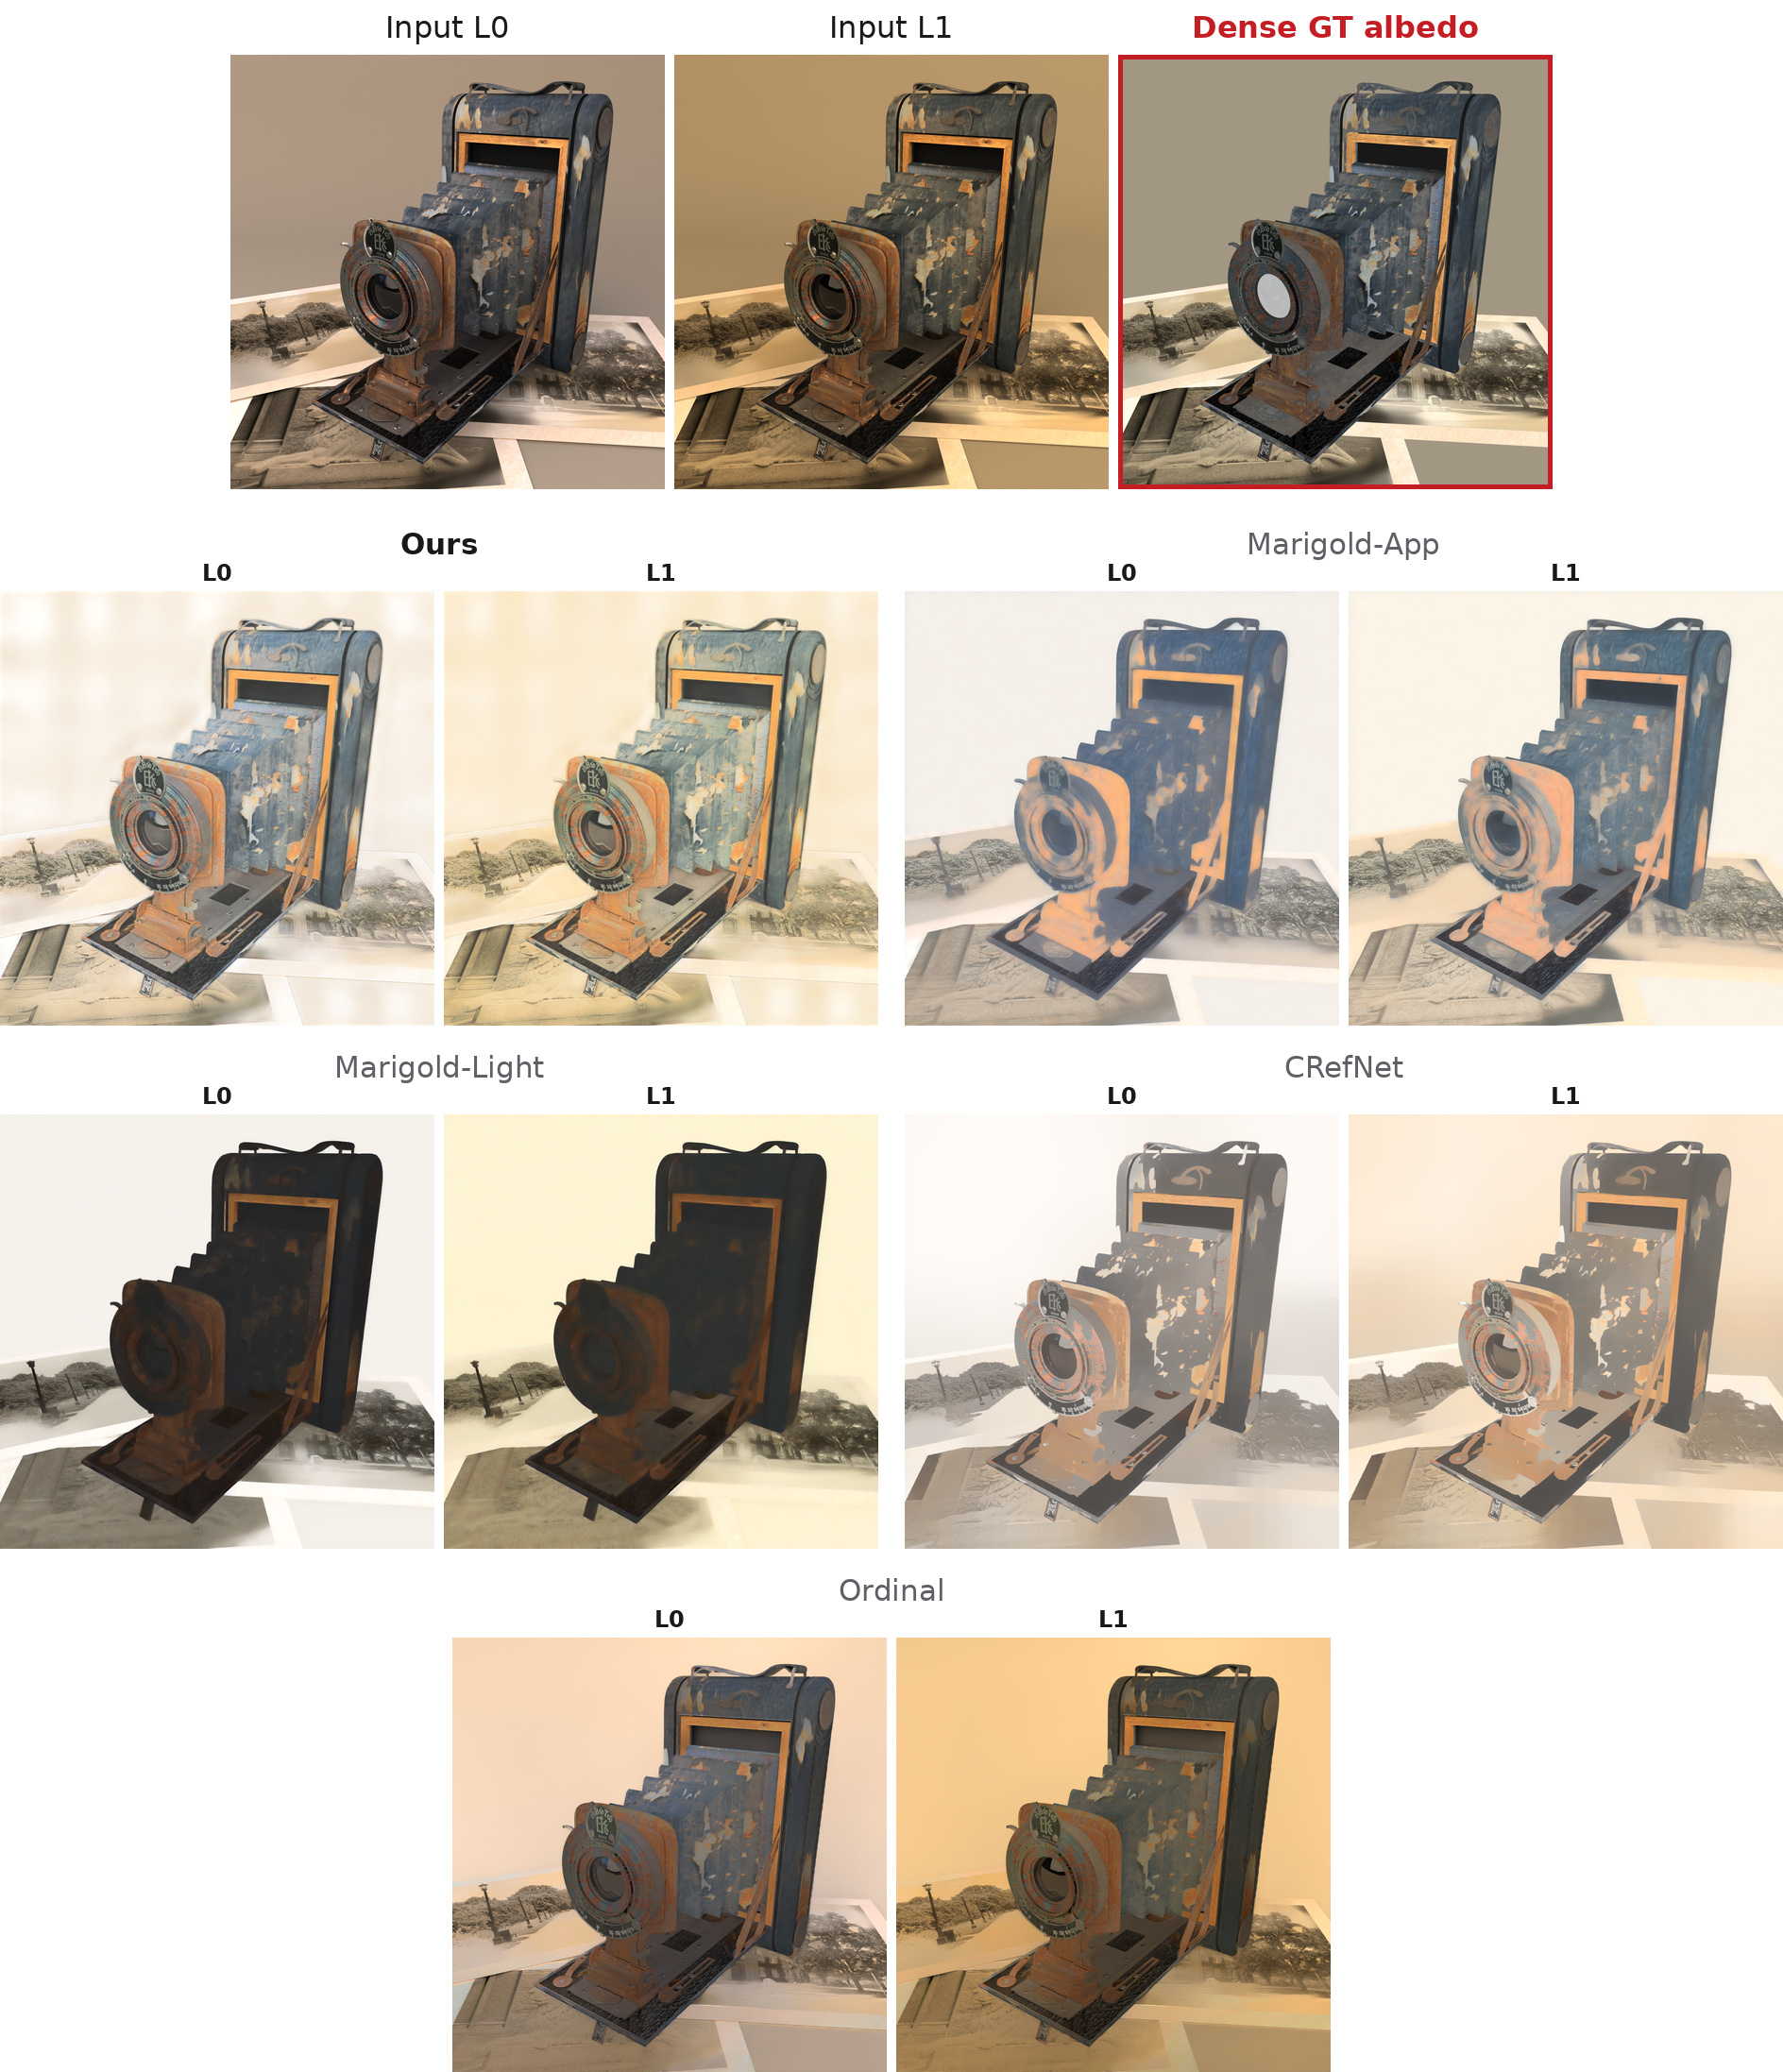
\includegraphics[width=0.98\textwidth]{images/hires/arap_model_grid.jpg}
  \caption[ARAP model comparison across illuminants on \emph{camera}.]{%
    Model-by-illuminant comparison on the ARAP \emph{camera} scene. The reference
    strip shows both rendered illuminant conditions and the dense ground-truth
    albedo once. The grid below shows each locally evaluated model's albedo under
    the same two illuminants, so the reader can compare consistency without
    repeatedly duplicating the reference. Predictions are independently
    scale-normalised for display, with no colour correction. The row labelled
    Ours uses the model selected for the thesis qualitative figures. The grid exposes
    different failure modes rather than declaring a winner: CRefNet suppresses
    much of the material colour, Marigold-Light and Ordinal retain illumination
    structure, and our L1 output still contains hard-shadow leakage. Marigold-App
    is comparatively stable on this scene; the full-set metrics in
    \tabref{tab:arap_constancy} and \tabref{tab:arap_accuracy} remain the
    aggregate evidence.
  }
  \label{fig:arap_models}
\end{figure}

\begin{figure}[t!]
  \centering
  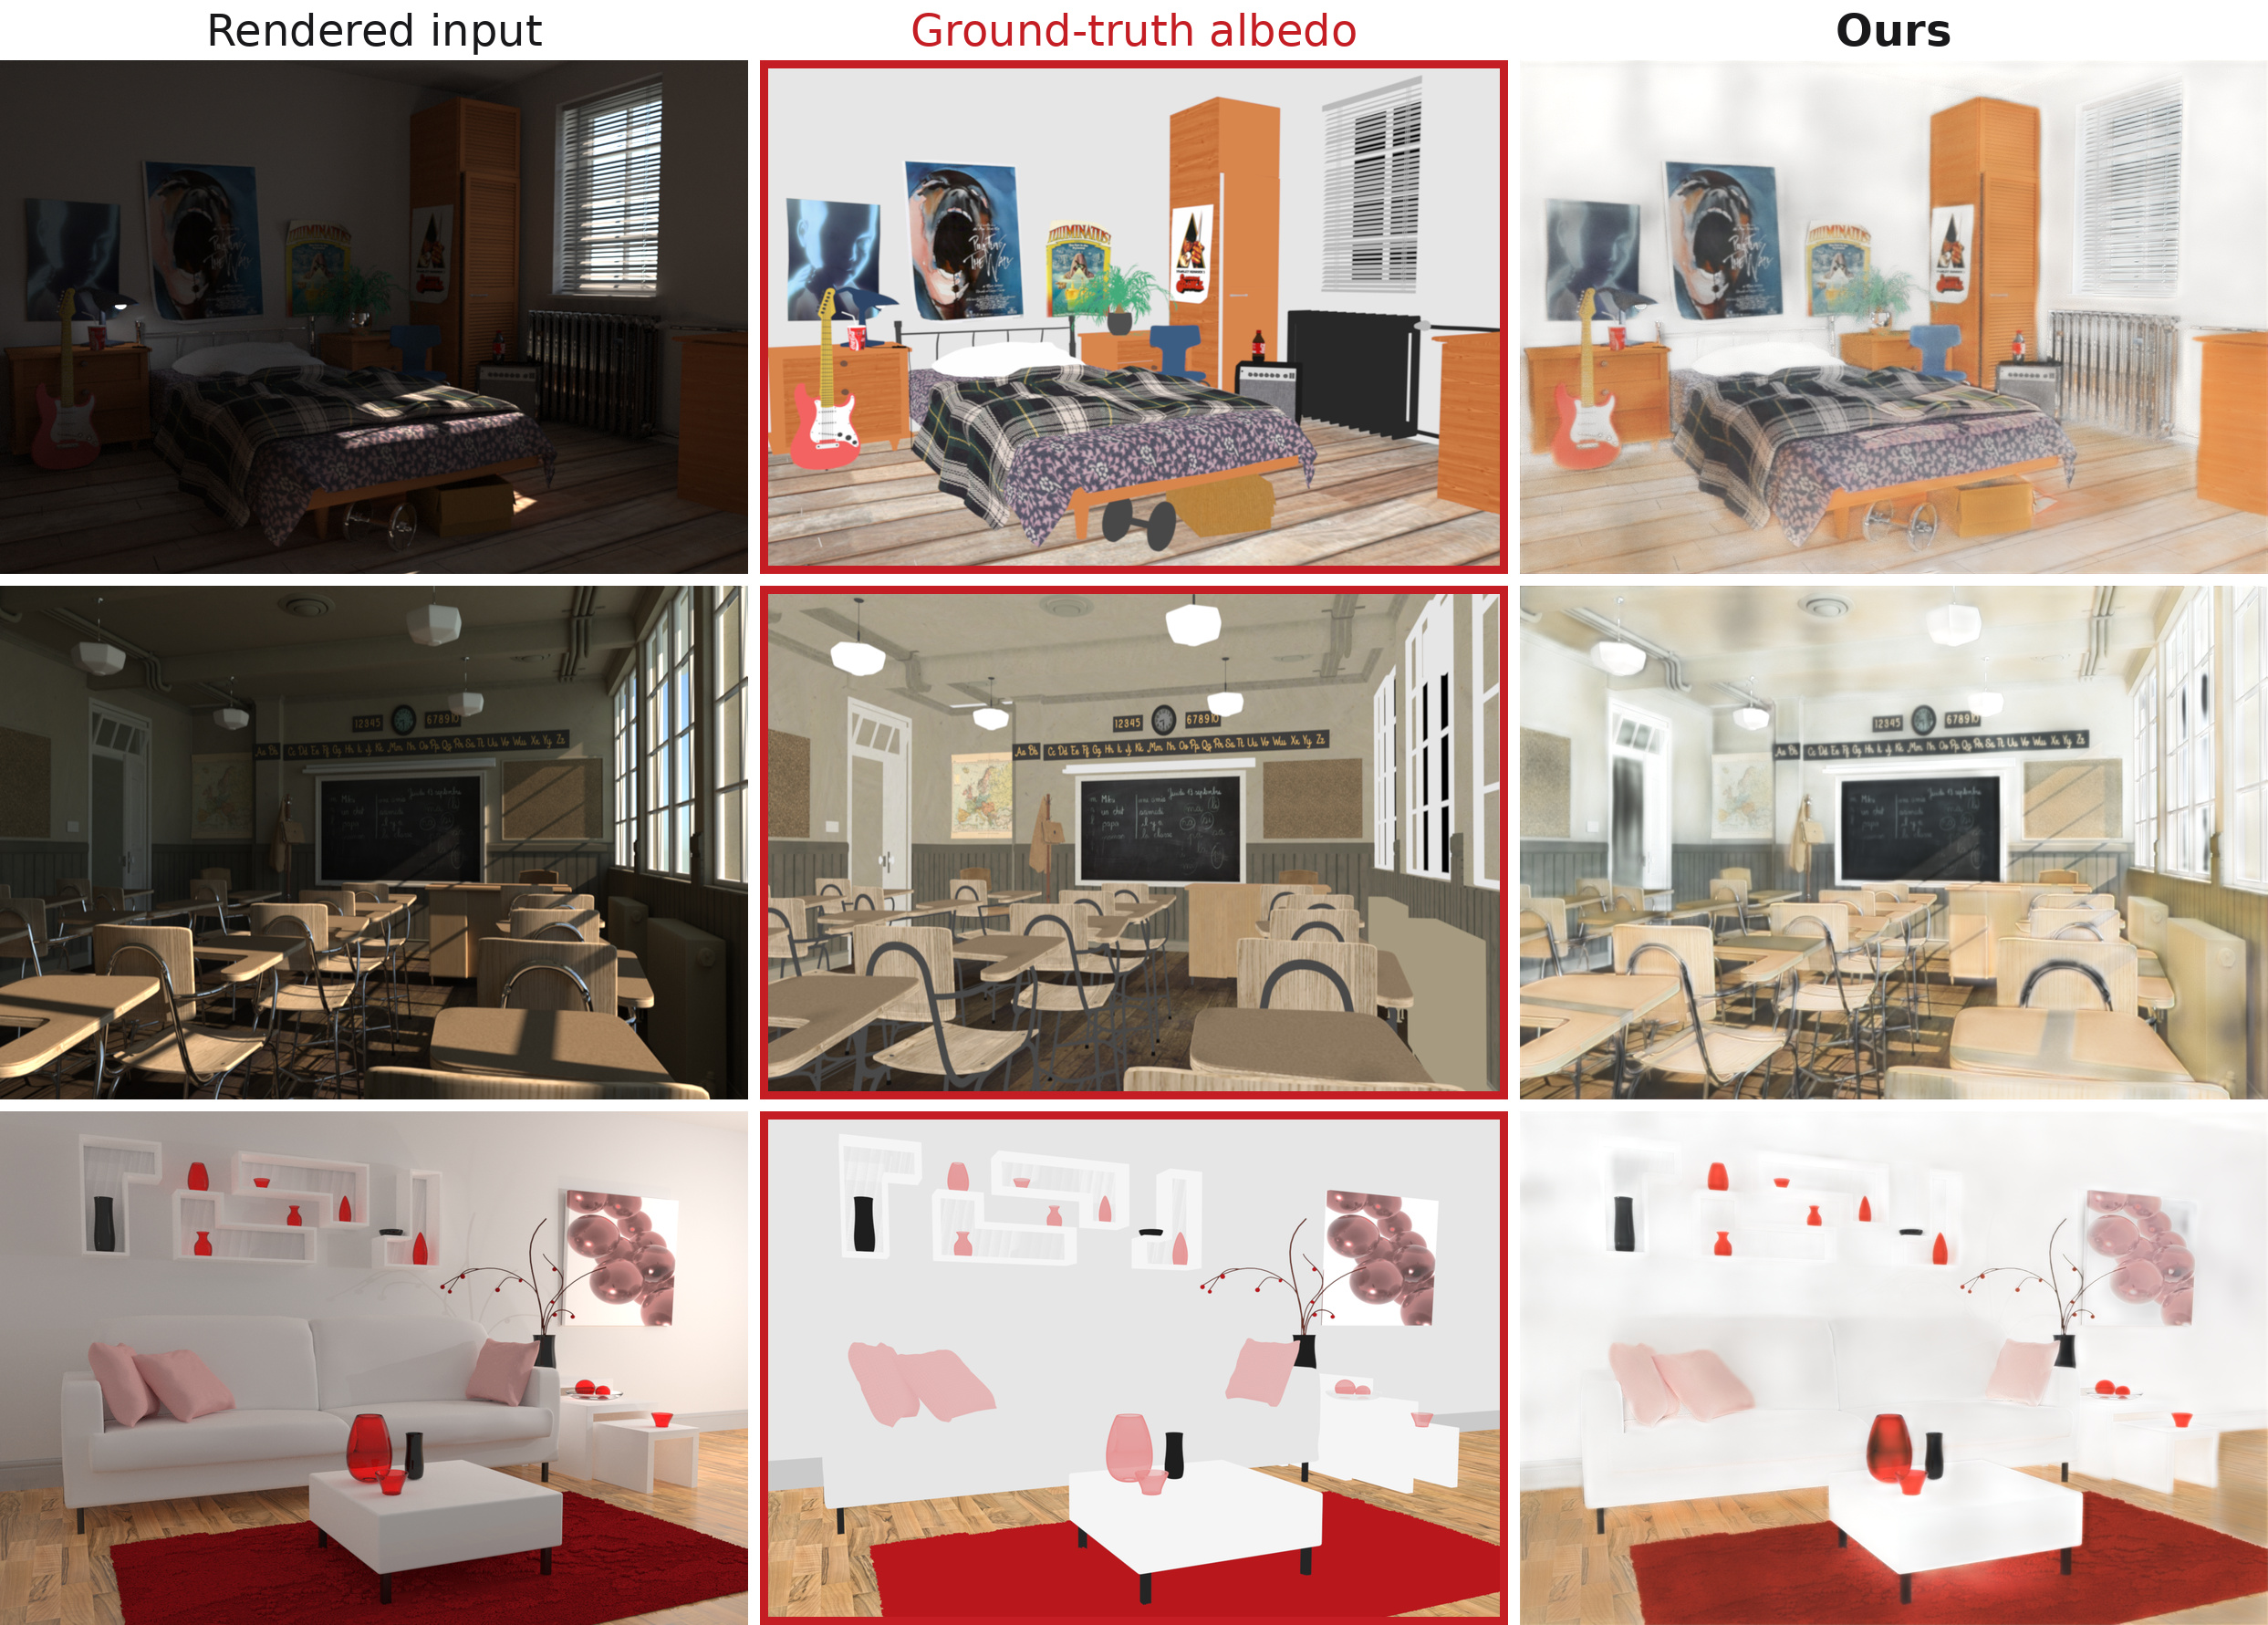
\includegraphics[width=\textwidth]{images/hires/arap_ours.jpg}
  \caption[ARAP qualitative accuracy on three indoor scenes.]{%
    Qualitative accuracy on three content-diverse ARAP scenes: \emph{bedroom},
    \emph{classroom}, and \emph{livingroom}. Each row shows the rendered input,
    dense ground-truth albedo (red border), and the prediction from Ours. This figure tests scene
    diversity and dense-albedo fidelity; \figref{fig:arap_models} separately
    compares models while the illuminant changes.
  }
  \label{fig:arap_constancy}
\end{figure}


\clearpage
\section{Ablation Study}
\label{sec:ablation}

The benchmark sections placed our model against external methods.
We now turn inward with one matched CARI study and one exploratory refinement study.
The first, the \emph{CARI ablation} of this section, asks whether the
constancy our model achieves genuinely comes from CARI, or from something
incidental; it isolates the two CARI components in a $2\times2$ ablation.
The second, the \emph{refinement study} of \secref{sec:lever_sweep}, takes
the resulting full-CARI model and asks whether it can be improved further, by
targeted extra loss terms or by the cross-illuminant training data of
\secref{sec:front3d}.
Together they explain both \emph{why} the model is built
the way it is and \emph{what} the cheaper alternatives cost.

The ablation isolates the contribution of CARI by comparing
configurations along two axes: whether the cross-render losses
($\mathcal{L}_{\text{inv}}$, $\mathcal{L}_{\text{expl}}$) are active, and
whether the colour-path bundle (wide RGB skip and its chroma-loss setting) is active
(\secref{sec:architecture}). These are the two components that, according to the coupling
argument in that section, are expected to interact.
\tabref{tab:ablation} summarises the resulting $2 \times 2$ design.
Part~1 reports self-consistency on raw-coloured inputs: the MID measures with their
fidelity guard, then ARAP constancy over all eligible groups and over the
domain-matched indoor subset. Part~2a reports measured-albedo accuracy, the
GT-achromatized ARAP accuracy guard, and ancillary IIW ordering. Part~2b reports
raw-input ARAP accuracy over the same all-ARAP and indoor subsets as Part~1. The
GT-achromatized ARAP columns support the within-study comparison but are not presented
as a reproduced published score.
All four configurations share the same 19k initialization, data curriculum,
and 40k training horizon. The two within-architecture comparisons are the
causal CARI tests: Row~1$\rightarrow$Row~2 toggles cross-render losses with
the colour path off, and Row~3$\rightarrow$Row~4 does the same with the colour
path on. These two within-architecture contrasts are the matched CARI tests.
The cross-axis colour-path comparison is not causal: it changes head parameters and
chroma supervision, starts Adam afresh, and the recorded fallback produces an
approximately $1.85\times$ different effective learning-rate trajectory. We therefore
report cross-axis differences descriptively rather than attributing them to the skip alone.

This ablation is also where the defect in the pooled chroma score of
\eqnref{eq:castrms} becomes visible, and we present it in that light because the
correction set out in \secref{sec:mid_results} was in fact discovered here. Under
\eqnref{eq:castrms}, Row~2 is the best configuration in the table because it attains the
lowest pooled cast of the four, while Row~4, the full model, is the worst. Inspection of
the predicted albedo contradicts this immediately: Row~2's albedo is visibly desaturated,
and Row~4's is not. The decomposition of \eqnref{eq:castdecomp} resolves the
contradiction. Row~2 retains only $0.484$ of the pseudo-GT between-material chroma
spread, so most of its low pooled score is the \emph{absence of colour}, not the absence
of drift. Once the drift is measured against the chroma each model actually carries
(\eqnref{eq:castrel}), the ordering reverses and Row~4 becomes the most invariant
configuration of the four.

\begin{table}[p]
  \caption[CARI ablation across constancy and accuracy.]{%
    CARI study across cross-render losses and the colour-path bundle. All
    configurations share the same 19k initialization and data
    curriculum, and 40k horizon; Row~1$\rightarrow$Row~2 and Row~3$\rightarrow$Row~4 are
    the matched cross-render comparisons. Cross-axis comparisons are descriptive because
    the colour path also changes chroma supervision, optimizer state, and effective
    learning-rate history.
    Part~1 reports raw-input constancy on the colour-varying ARAP groups (the same
    $16$/$11$ subset used in \tabref{tab:arap_constancy} and \tabref{tab:lever_sweep});
    Part~2a measured-albedo accuracy, the
    GT-achromatized ARAP guard and ancillary IIW ordering; Part~2b raw-input ARAP accuracy.
    Lower is better everywhere except ARAP SSIM, and the aggregate spread ratio, whose
    target is $1.000$. Best per column is \textbf{bold}.
    \figref{fig:ablation} shows the corresponding albedo and variation maps.
  }
  \label{tab:ablation}
  \centering
  \textbf{\small Part 1: Raw-input constancy (self-consistency across illuminants)}\\[2pt]
  \resizebox{\textwidth}{!}{%
  \begin{tabular}{@{}lllcccccccc@{}}
    \toprule
    & & & \multicolumn{4}{c}{MID (30 scenes)} & \multicolumn{2}{c}{ARAP all (col.\ varying, $n{=}16$)}
        & \multicolumn{2}{c}{ARAP indoor (col.\ varying, $n{=}11$)} \\
    \cmidrule(lr){4-7}\cmidrule(lr){8-9}\cmidrule(l){10-11}
    Row & Cross-render & Colour path
        & $C_{\text{mat}}$ $\downarrow$ & $\text{Cast}_{\text{rel}}$ $\downarrow$
        & $\text{Chroma}_{\text{err}}$ $\downarrow$ & Spread ratio ($\to 1$)
        & $C_{\text{arap}}$ $\downarrow$ & $\text{Cast}_{\text{RMS}}^{\S}$
        & $C_{\text{arap}}$ $\downarrow$ & $\text{Cast}_{\text{RMS}}^{\S}$ \\
    \midrule
    1 & off & off & 0.250 & 0.477 & 0.186 & 0.512 & 0.164 & 0.102 & 0.122 & 0.105 \\
    2 & on  & off & 0.180 & 0.447 & 0.201 & 0.484 & \textbf{0.145} & \textit{0.080} & \textbf{0.108} & \textit{0.085} \\
    3 & off & on  & 0.259 & 0.444 & \textbf{0.124} & 0.925 & 0.155 & 0.106 & 0.117 & 0.105 \\
    4 & on  & on  & \textbf{0.157} & \textbf{0.425} & 0.129 & \textbf{0.999} & 0.154 & 0.092 & 0.119 & 0.094 \\
    \bottomrule
  \end{tabular}}\\[3pt]
  {\footnotesize MID spread ratios use the ratio of aggregate predicted and pseudo-GT
  spreads, not the biased mean of per-scene ratios. The ARAP $\text{Cast}_{\text{RMS}}$ columns
  carry no between-material term but are still \emph{absolute} chroma variances, which a
  colourless albedo also minimises.}\\[4pt]
  \textbf{\small Part 2a: Standard-protocol accuracy and structure (against ground truth)}\\[2pt]
  \resizebox{\textwidth}{!}{%
  \begin{tabular}{@{}lllcccccc@{}}
    \toprule
    & & & \multicolumn{2}{c}{MAW} & \multicolumn{3}{c}{ARAP (GT-achromatized)} & \multicolumn{1}{c}{IIW} \\
    \cmidrule(lr){4-5}\cmidrule(lr){6-8}\cmidrule(l){9-9}
    Row & Cross-render & Colour path & $\Delta E$ $\downarrow$ & Int.$\times$100 $\downarrow$ & LMSE$^\dagger$ $\downarrow$ & mn-RMSE$^\dagger$ $\downarrow$ & SSIM$^\dagger$ $\uparrow$ & WHDR $\downarrow$ \\
    \midrule
    1 & off & off & 4.434 & 0.409 & 0.0307 & 0.2378 & 0.8055 & 0.334 \\
    2 & on  & off & 4.631 & 0.474 & 0.0320 & 0.2313 & \textbf{0.8069} & \textbf{0.283} \\
    3 & off & on  & \textbf{4.115} & \textbf{0.395} & 0.0283 & 0.2348 & 0.8047 & 0.327 \\
    4 & on  & on  & 4.155 & 0.504 & \textbf{0.0279} & \textbf{0.2259} & 0.8067 & 0.286 \\
    \bottomrule
  \end{tabular}}\\[5pt]
  \textbf{\small Part 2b: Raw-input ARAP albedo accuracy (against ground truth)}\\[2pt]
  \resizebox{\textwidth}{!}{%
  \begin{tabular}{@{}lllcccc@{}}
    \toprule
    & & & \multicolumn{2}{c}{All ARAP (raw input)}
        & \multicolumn{2}{c}{Indoor ARAP (raw input)} \\
    \cmidrule(lr){4-5}\cmidrule(l){6-7}
    Row & Cross-render & Colour path
        & LMSE $^\ddagger$ $\downarrow$ & mn-RMSE $^\ddagger$ $\downarrow$
        & LMSE $^\ddagger$ $\downarrow$ & mn-RMSE $^\ddagger$ $\downarrow$ \\
    \midrule
    1 & off & off & 0.0463 & 0.341 & 0.0441 & 0.323 \\
    2 & on  & off & 0.0397 & \textbf{0.292} & \textbf{0.0370} & \textbf{0.275} \\
    3 & off & on  & 0.0426 & 0.319 & 0.0400 & 0.301 \\
    4 & on  & on  & \textbf{0.0396} & 0.293 & 0.0382 & 0.276 \\
    \bottomrule
  \end{tabular}}\\[3pt]
  {\footnotesize $\dagger$ GT-achromatized ARAP accuracy guard (136 of 157 images): an internal
  within-study comparison, not a reproduced literature table. IIW WHDR is ancillary and is
  not a selection criterion. $\ddagger$ Raw-input ARAP accuracy is a local multi-illuminant
  stress test and is not compared with published white-balanced results.}
\end{table}

\paragraph{Effect of cross-render losses within each architecture}
The clean CARI comparisons are Row~1$\rightarrow$Row~2 and
Row~3$\rightarrow$Row~4, the two contrasts in which only the cross-render losses change.
The clearest effect is on \emph{lightness} stability: cross-render supervision lowers
$C_{\text{mat}}$ from 0.250 to 0.180 with the colour path off and from 0.259 to 0.157 with
it on, corresponding to a $28\%$ and $39\%$ reduction, both well outside the scene-bootstrap intervals of
\tabref{tab:mid}. On scale-normalised hue invariance the effect is present but small:
$\text{Cast}_{\text{rel}}$ moves from 0.477 to 0.447 and from 0.444 to 0.425.
The relevant paired bootstrap, rather than overlap of marginal intervals, gives
Row~1-minus-Row~2 $0.030$ with a $95\%$ interval $[0.011,0.049]$, and
Row~3-minus-Row~4 $0.019$ with interval $[0.007,0.031]$. Both are modest but
significant hue-stability gains.

The pseudo-GT calibration guard supplies the necessary qualification. With the colour
path off, $\text{Chroma}_{\text{err}}$ worsens from 0.186 to 0.201; with it on, the
change from 0.124 to 0.129 is not significant. CARI therefore improves paired
constancy but does not itself improve colour calibration. It also improves ancillary
IIW WHDR in the first pair, while both MAW measures worsen slightly. The load-bearing
result is the repeated paired constancy gain, read beside rather than instead of the
external accuracy guards.

\paragraph{Association with the colour-path bundle}
The colour-path rows retain $92.5\%$ and $99.9\%$ of the pseudo-GT aggregate chroma
spread, while the rows without it retain $51.2\%$ and $48.4\%$. They also have lower
$\text{Chroma}_{\text{err}}$ and stronger MAW colour, with Row~3 obtaining the best
$\Delta E$ (4.115) and intensity score (0.395). This is strong descriptive evidence
that the bundle preserves colour. It is not a skip-only causal estimate because the
bundle changes chroma supervision, head parameters, optimizer state, and effective
learning-rate history.

This is the opposite of what the pooled score reports, and the discrepancy is instructive
rather than awkward. Under \eqnref{eq:castrms} the colour-skip rows appear to
\emph{double} their chroma cast (0.287 to 0.519, 0.268 to 0.555); under
\eqnref{eq:castdecomp} that increase is almost entirely the between-material term
$S(A)$ rising from roughly $0.25$ to roughly $0.48$ as the model recovers the chromatic
diversity that the ground-truth albedo actually possesses ($S(A^{*}) = 0.495$). The
pooled metric was charging the model for the colour it restored relative to the
pseudo-reference. Row~4 is
consequently the strongest configuration in the table on both constancy axes,
$C_{\text{mat}}$ and $\text{Cast}_{\text{rel}}$, and is not the weakest, contrary to what
the superseded score indicated.

\paragraph{Role of IIW and ARAP in the next study}
IIW WHDR is a sparse perceptual ordinal measure; it is therefore retained as
a complementary column rather than the colour-constancy selection criterion. Its Row~2 result is
consistent with the real cross-render signal helping ordinal reflectance, but
does not establish that transfer on its own. ARAP varies less across the four
rows than MID: all-ARAP $C_{\text{arap}}$ spans 0.145--0.164 and indoor-ARAP
0.108--0.122, while the corresponding MID $C_{\text{mat}}$ range is 0.157--0.259.
This limited ARAP response motivates
testing a synthetic cross-render source in the next ablation; it is a
hypothesis motivated by the measured domain difference, not a conclusion about
its cause.

\paragraph{Why Row 4 initializes Table B}
Row~4 is used as the Table-B starting point because it is the complete CARI
configuration and, on the corrected metrics, the strongest of the four rows on both
constancy axes while retaining $99.9\%$ of the pseudo-GT aggregate chroma spread.
Its residual weaknesses (a slightly higher $\text{Chroma}_{\text{err}}$ than Row~3
(0.129 against 0.124) and a marginally worse MAW $\Delta E$
(4.155 against 4.115)) remain explicit in \tabref{tab:ablation} and inform the next
study's ARAP--MAW selection criteria.

\figref{fig:ablation} shows the qualitative effect of each ablation row.

\begin{figure}[t!]
  \centering
  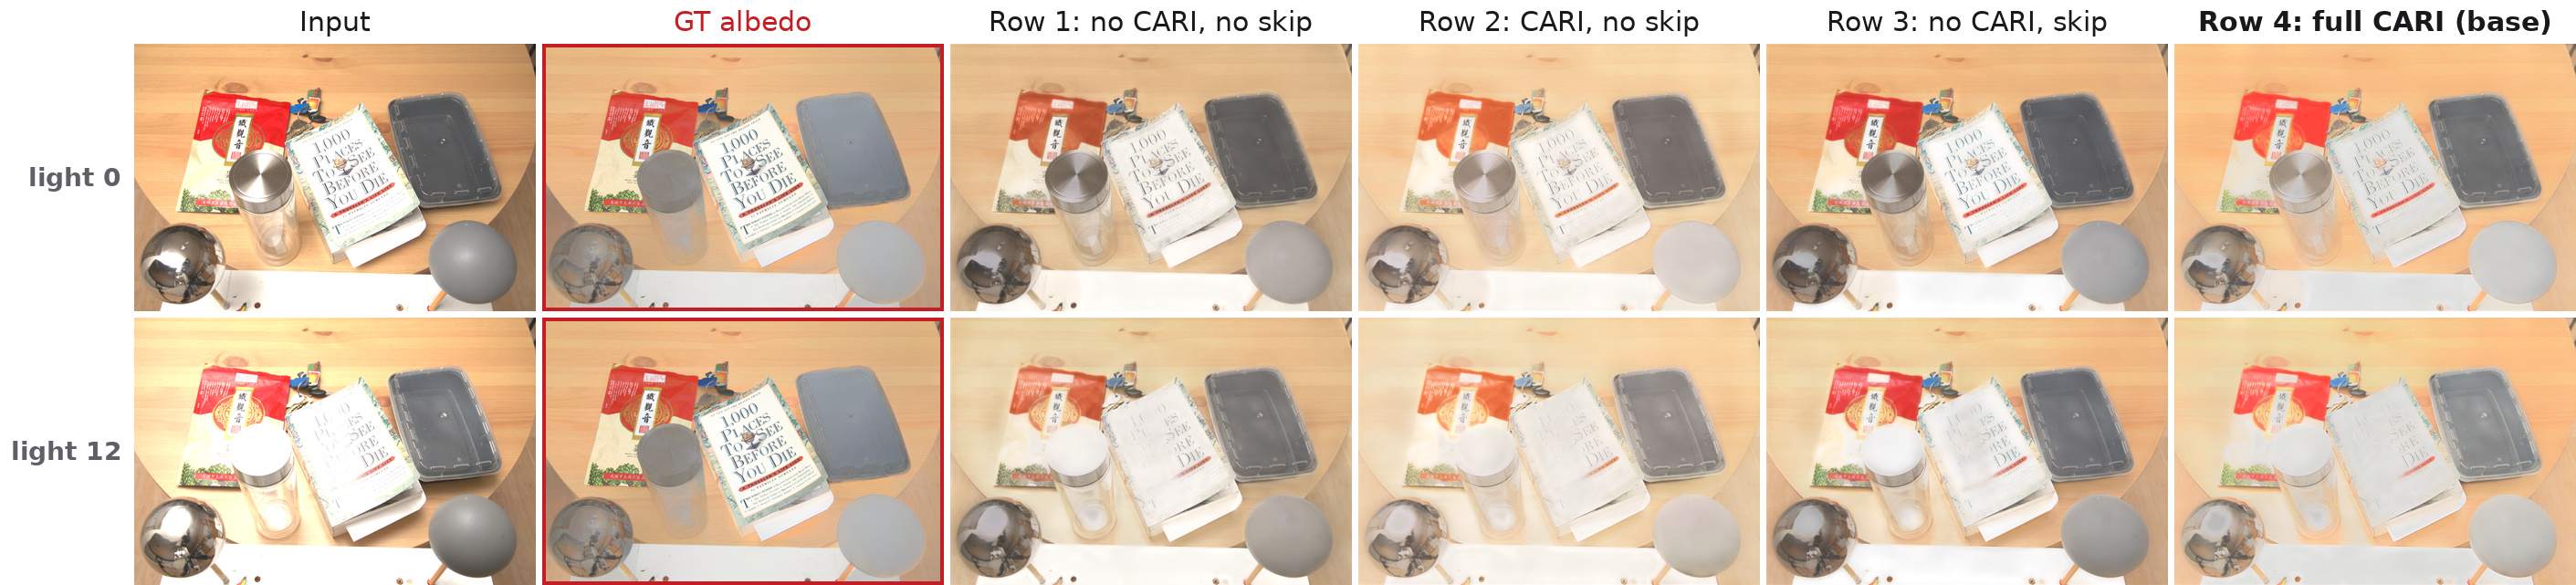
\includegraphics[width=\textwidth]{images/hires/ablation_mid.jpg}
  \caption[Qualitative CARI ablation on MID.]{%
    Ablation: the four CARI configurations on one MID scene under three
    illuminant conditions (L0, L10, L20).
    Columns: the three input conditions, the pseudo-ground-truth albedo (red
    box), the three predicted albedos, and two cross-condition variation
    heatmaps computed across five illuminant conditions (L0, L5, \ldots, L20;
    5, three of which are shown): luminance CoV, matching MID
    $C_{\text{mat}}$, and the legacy pooled chroma-cast CoV diagnostic
    $\text{Cast}_{\text{RMS}}$ ($\sqrt{\mathrm{Var}(R/G) + \mathrm{Var}(B/G)}$
    across conditions).
    Rows, top to bottom: no CARI (Row~1), cross-render only (Row~2), colour-skip
    only (Row~3), and full CARI (Row~4).
    These are local, single-scene illustrations rather than estimates of the
    full-split metrics in \tabref{tab:ablation}: the heatmaps expose where the
    predicted albedo changes with illumination, while the table establishes the
    dataset-level ranking. In particular, chroma variation is spatially and
    scene dependent, so the figure is not used to infer the global
    $\text{Cast}_{\text{RMS}}$ ordering.
  }
  \label{fig:ablation}
\end{figure}


\section{Refinement Study: Loss Levers versus Cross-Illuminant Data}
\label{sec:lever_sweep}

The ablation established that CARI works. This study asks the natural follow-up:
can the full-CARI model be pushed further, and if so, by \emph{what kind} of
intervention?
Two candidates are available, and they are of fundamentally different types.
The first is a pair of extra \emph{loss terms} (``levers''), each targeting a
residual weakness visible in the full-CARI albedo: smooth shading ramps that
survive on flat surfaces, and shadow boundaries that leak into the albedo.
The second is more \emph{data}, specifically the 3D-Front-IID corpus
(\secref{sec:front3d}), which supplies the wide, deliberately coloured
illuminant changes that neither Hypersim nor MID provides.
Running both in one controlled study lets us ask a question neither could
answer alone: if the levers are compensating for a signal missing from the
training data, then supplying that signal should reduce or remove the need for
them.

\paragraph{The two loss levers}
Writing $\mathbf{A}$ and $\mathbf{S}_d$ for the predicted albedo and diffuse
shading and $\mathbf{I}$ for the input:

\begin{itemize}
  \item \textbf{Flatness} (\emph{flat}): a chroma-gated low-frequency
        albedo-flatness prior. With $\mathbf{A}_{\text{LF}}$ a low-pass of the
        predicted albedo and $w_c$ a per-pixel gate that is high only where the
        local chromaticity is uniform (same material),
        $\mathcal{L}_{\text{flat}} = \sum_p w_c(p)\,\lVert \nabla
        \mathbf{A}_{\text{LF}}(p) \rVert_1$.
        It removes smooth shading ramps left in the albedo while the chroma
        gate preserves genuine material and texture edges.
  \item \textbf{Shadow-invariance} (\emph{sh\_inv}): a manufactured-shadow
        self-supervision. A smooth synthetic relighting field $\sigma$ is cast
        onto a Hypersim image, and the predicted albedo is required to be
        invariant to it:
        $\mathcal{L}_{\text{sh\_inv}} = \lVert \mathbf{A}(\mathbf{I} \odot
        \sigma) - \mathbf{A}(\mathbf{I}) \rVert_1$.
\end{itemize}

The synthetic relighting used by the shadow lever is shown in
\figref{fig:shadow_aug}. This branch is separate from CARI: CARI's
$\mathcal{L}_{\text{inv}}$ uses real MID raw pairs, whereas the shadow lever
manufactures a second observation on Hypersim with a \emph{known} field and
applies only $\mathcal{L}_{\text{sh\_inv}}$.
The distinction matters for the reading below: the shadow lever is a synthetic
stand-in for exactly the kind of second observation that 3D-Front-IID provides
for real.

\begin{figure}[t!]
  \centering
  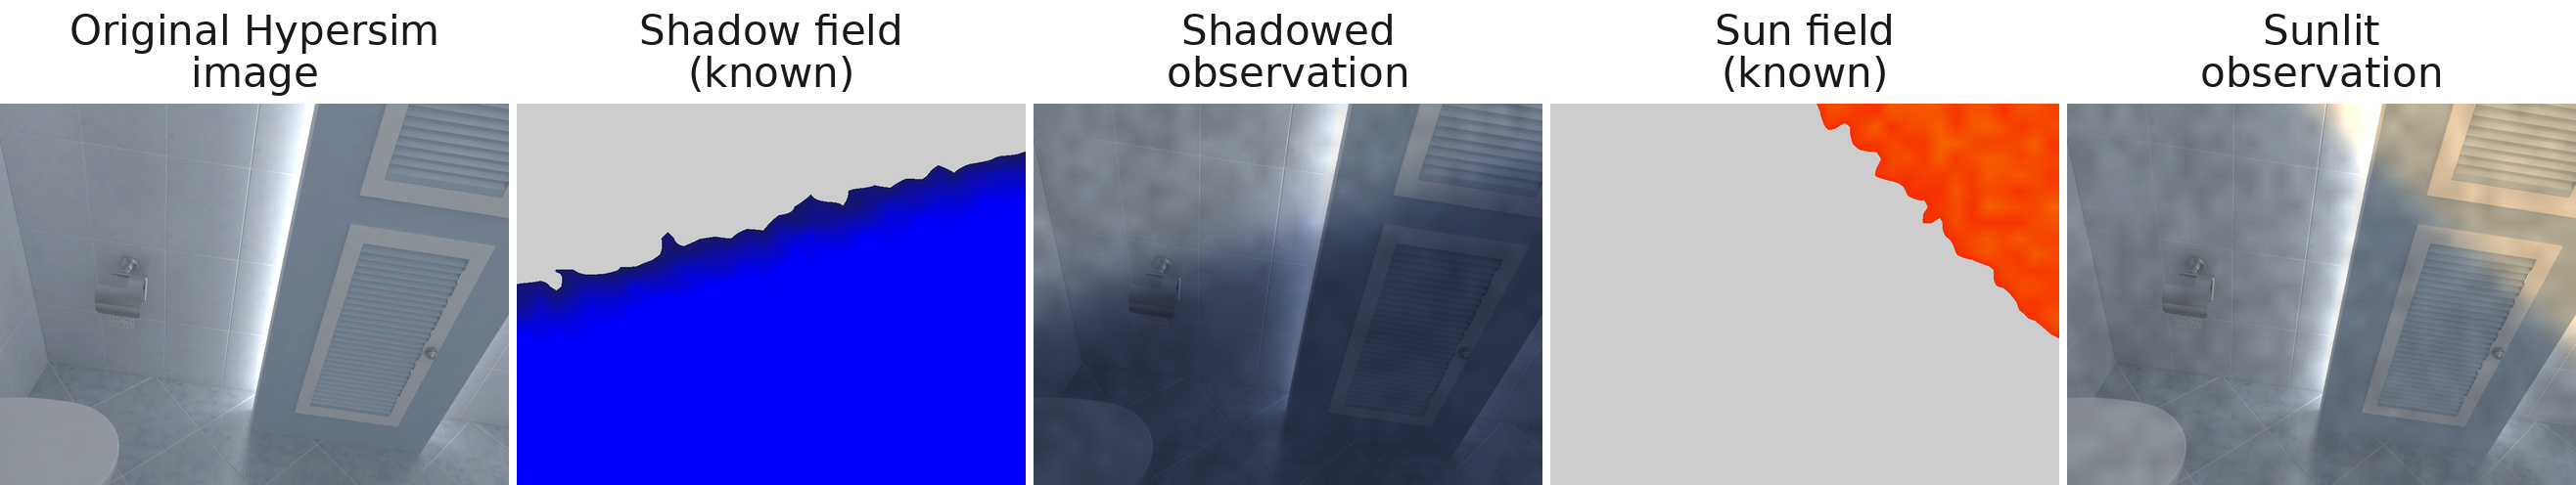
\includegraphics[width=\textwidth]{images/hires/shadow_aug.jpg}
  \caption[Synthetic relighting for shadow invariance.]{%
    Synthetic relighting used by the shadow-invariance lever.
    A known multiplicative field is applied to a Hypersim image to manufacture a
    shadowed or sunlit second observation, and the predicted albedo is required
    to stay invariant under it.
    This loss is distinct from CARI's real-pair invariance loss, and it is the
    manufactured counterpart of the genuine cross-illuminant pairs supplied by
    3D-Front-IID (\secref{sec:front3d}).
  }
  \label{fig:shadow_aug}
\end{figure}

\paragraph{Design}
Every row of \tabref{tab:lever_sweep} starts from the same full-CARI checkpoint
(Row~4 of \tabref{tab:ablation} at 40k iterations) and trains for a
further 20k iterations to a 60k horizon, at the same constant learning rate.
The rows share initialization, horizon, and learning rate, but the logged data
mixtures are not identical. Rows~1--2 use Hypersim/MID/InteriorVerse weights
$0.4/0.3/0.3$; Row~3 changes mixture during training before ending at
$0.3/0.3/0.15/0.25$ with 3D-Front-IID; Row~4 uses that standardized mix; and
Row~5 uses approximately $0.32/0.24/0.24/0.20$ throughout. Current YAML files do
not retroactively define these checkpoints, so this provenance comes from the logs.
Row~1 is the zero-lever control: it receives the identical 20k iterations of
extra training with neither intervention, so every other row is read against it
rather than against the base checkpoint, and the effect of the extra training
itself is not mistaken for the effect of a lever or a dataset.
Row~2 adds the two levers. Row~3 instead adds 3D-Front-IID, with both lever
weights explicitly zero, isolating the data axis.
Rows~4 and~5 add levers, but their recorded mixtures differ. Consequently only
Rows~1$\rightarrow$2 is a matched lever contrast. The 3D-Front and flatness
comparisons are exploratory associations rather than single-variable ablations.
A no-regression gate, specified in the training configuration before the runs, applies
throughout: an intervention is kept only if it does not regress the coloured-illuminant
constancy metrics or the albedo-accuracy guard by more than approximately 10\% relative to
the control. We describe it as pre-specified rather than pre-registered: it is fixed in the
config, not lodged as a timestamped artefact ahead of the results.

\begin{table}[t!]
  \caption[Refinement study across loss and data configurations.]{%
    Refinement study. All rows resume the same full-CARI checkpoint
    (\tabref{tab:ablation}, Row~4, at 40k) and train a further 20k iterations to
    60k at the same learning rate. Only Rows~1$\rightarrow$2 is a matched contrast;
    the 3D-Front rows have the logged mixture histories stated above and are interpreted
    exploratorily.
    Lower is better on every column. Guards are not used for selection: the gate
    is applied to the constancy columns and MAW $\Delta E$.
  }
  \label{tab:lever_sweep}
  \centering
  \resizebox{\textwidth}{!}{%
  \begin{tabular}{@{}lllccccccccc@{}}
    \toprule
    & & & \multicolumn{3}{c}{MID} & \multicolumn{2}{c}{ARAP indoor (col.\ varying)}
        & \multicolumn{2}{c}{MAW} & \multicolumn{2}{c}{Guards} \\
    \cmidrule(lr){4-6}\cmidrule(lr){7-8}\cmidrule(lr){9-10}\cmidrule(l){11-12}
    Row & Configuration & Levers
        & $C_{\text{mat}}$ $\downarrow$ & $\text{Cast}_{\text{rel}}$ $\downarrow$
        & $\text{Chroma}_{\text{err}}$ $\downarrow$
        & $C_{\text{arap}}$ $\downarrow$ & $\text{Cast}_{\text{RMS}}$ $\downarrow$
        & $\Delta E$ $\downarrow$ & Int.$\times$100 $\downarrow$
        & mn-RMSE $\downarrow$ & WHDR $\downarrow$ \\
    \midrule
    1 & Control (extra training only) & --                      & 0.161 & 0.415 & \textbf{0.115} & 0.116 & 0.090 & 4.179 & \textbf{0.511} & 0.2194 & 0.283 \\
    2 & \quad + levers                & flat, sh\_inv           & 0.146 & 0.426 & \textbf{0.115} & 0.100 & 0.085 & 4.193 & 0.732 & \textbf{0.2099} & 0.281 \\
    3 & \quad + 3D-Front-IID          & --                      & 0.163 & 0.418 & 0.120 & 0.111 & 0.080 & 4.040 & 0.512 & 0.2274 & 0.280 \\
    4 & \quad + 3D-Front + levers     & flat (reduced), sh\_inv & \textbf{0.130} & 0.421 & 0.121 & \textbf{0.096} & \textbf{0.077} & \textbf{3.981} & 0.624 & 0.2150 & \textbf{0.264} \\
    5 & \quad + 3D-Front + levers     & flat (full), sh\_inv    & 0.149 & 0.421 & 0.143 & 0.097 & 0.078 & 4.231 & 0.719 & 0.2103 & 0.282 \\
    \bottomrule
  \end{tabular}}\\[4pt]
  {\footnotesize Guard columns (ARAP mn-RMSE, IIW WHDR) are reported for
  transparency and are not
  selection criteria: IIW WHDR is a sparse perceptual ordinal measure with a
  different target from colour constancy
  (\secref{sec:iiw_results}).
  $\text{Cast}_{\text{rel}}$ is deliberately \emph{not} bolded: its five values span
  0.415--0.426, a range of 2.6\%, and no row is meaningfully more illuminant-invariant
  than any other. That column is a null result and is discussed as such.}
\end{table}

\paragraph{What the comparison can establish}
Rows~1$\rightarrow$2 establish the effect of the two levers under the no-3D-Front
mixture. The remaining rows support model selection and hypothesis generation, not
component attribution, because their mixture histories differ. The selected
configuration is therefore the best observed gate-passing trade-off, reported
alongside the full-CARI starting point rather than replacing it silently.

\paragraph{Illuminant invariance does not move}
The first result of the study is a negative one, and it is reported first because it
constrains how everything else may be read. Neither intervention changes illuminant
invariance. $\text{Cast}_{\text{rel}}$ takes the values 0.415, 0.426, 0.418, 0.421 and
0.421 across the five rows, a spread of 2.6\%, with the zero-lever control among the
best and the two combined rows indistinguishable from it. Whatever the levers and the
3D-Front-IID corpus contribute, they do not make the albedo more stable under a change of
illuminant than twenty thousand further iterations of ordinary training would have.

This is worth stating plainly because the superseded pooled score would have suggested
otherwise. Under \eqnref{eq:castrms} the same five rows span 0.523 to 0.586, a 12\%
range, and appear to rank cleanly. That apparent ranking is the between-material term of
\eqnref{eq:castdecomp}, not drift: Row~5 (the full-strength flatness prior) posts
the worst pooled cast of the five (0.586) purely because it is the most over-saturated row
in the table; its aggregate spread ratio is 1.055, while Row~4 retains 0.941.
The pooled score was ranking the rows partly by how much albedo
chroma each carried. Once that term is removed, the constancy axis is flat, and the study
must be adjudicated on the axes that do respond.

\paragraph{What does respond: chroma fidelity, lightness stability, and measured colour}
The rows are not inert; they move calibration, lightness stability, and measured colour.
Row~4 has the best lightness stability ($C_{\text{mat}}=0.130$), MAW colour
($\Delta E=3.981$), coloured-illuminant ARAP scores (0.096/0.077), and IIW ordering
(0.264). Its MID $\text{Chroma}_{\text{err}}=0.121$ is slightly worse than the
0.115 controls, and its MAW intensity score is also worse, so selection is a trade-off
rather than a clean sweep.

Row~5 is associated with worse pseudo-GT calibration
($\text{Chroma}_{\text{err}}=0.143$), lightness stability (0.149), and MAW
$\Delta E$ (4.231) than Row~4. Because its data mix also differs, this cannot isolate
the full flatness weight as the cause. The matched Rows~1$\rightarrow$2 comparison shows
that the levers improve $C_{\text{mat}}$ and the ARAP guard while worsening MAW
intensity; Row~3 shows that the 3D-Front configuration can improve MAW colour without
improving MID lightness stability. The combined Row~4 is retained as the best observed
compromise, not as proof of complementary causal effects.

Row~4 is therefore the selected configuration and is the model reported as
\emph{Ours} throughout \secref{sec:mid_results}--\secref{sec:arap_results}.
